\chapter{\MakeUppercase{NCTM Case Study}}
The National Center for Therapeutic Medicine (NCTM) was used as a test
bed for the original methodology. NCTM is a building located on the
campus of Texas A\&M University, in College Station, Texas. 

The National Center for Therapeutics Manufacturing (NCTM) combines the
educational and manufacturing focuses of the biopharmaceutical industry.
The NCTM building is approximately 150,000 ft\textsuperscript{2} with
nearly 50,000 ft\textsuperscript{2} of educational facilities that
include wet labs, culture facilities, large lecture halls, and a mock
current Good Manufacturing Practice (cGMP) training suite. Around
120,000 ft\textsuperscript{2} is on the first level and 30,000
ft\textsuperscript{2} is on the second level. 

The cGMP Suite contains modern biopharmaceutical manufacturing equipment
that students can use to learn industry practices. The wet labs are
equipped with chemical fume hoods and the necessary electronic equipment
for following standard operating procedures used in the
biopharmaceutical industry. The lecture halls seat up to 120 students
and have large floor to ceiling windows. There is also an Apple Computer
laboratory with 48 workstations on the second floor. 

On the academic side, three dedicated outdoor air handling
units (OAHU) serve seven child air handling units. Two of the air handling
units are constant speed, and the others are variable air volume. OAHU
1-1 serves its wet lab and also feeds into AHU 1-1 and AHU 1-2. OAHU
1-2 serves AHU 1-3 and 1-4 on the first floor. OAHU 2-1 serves three
children air handlers on the second floor, AHU 2-1, 2-2, and 2-3. 

This document focuses on the academic side of the building since
Utilities and Energy services with Texas A\&M University are only
allowed to make immediate changes to the HVAC system on this side. In
summary, the relavent parameters concerning NCTM are that it houses
several biopharmaceutical labs, it has an academic side that can be
immediately changed and a manufacturing side that cannot be immediately
changed, and relies on dedicated outdoor air handling units to pretreat
outdoor air. 


\begin{table}
\centering
\caption{Occupied/Unoccupied scheduling for the AHUs as described.}
\label{tab:OnOffSched}
\begin{tabular}{l c c c}
\toprule
Level          & OAHU     & AHU \#  & AHU Schedule    \\
\midrule
Floor 1 Area B & OAHU 1-1 & N/A     & 24/7            \\
Floor 1 Area B & OAHU 1-1 & AHU 1-1 & 24/7            \\
Floor 1 Area B & OAHU 1-1 & AHU 1-2 & 6am - 6pm, M-F  \\
Floor 1 Area A & OAHU 1-2 & AHU 1-3 & 6am - 8pm, M-F  \\
Floor 1 Area A & OAHU 1-2 & AHU 1-4 & 6am - 8pm, M-F  \\
Floor 2        & OAHU 2-1 & AHU 2-1 & 6am - 10pm, M-F \\
Floor 2        & OAHU 2-1 & AHU 2-2 & 6am - 10pm, M-F \\
Floor 2        & OAHU 2-1 & AHU 2-3 & 6am - 10pm, M-F \\
\bottomrule
\end{tabular}
\end{table}

\begin{figure}
    \centering
\includegraphics[]{Plots/TempRiseVsFlow-AHU-2-14.pdf}
\caption{Temperature rise due to the mixing of plenum air at the terminal unit for FPVAV-2-14. }
\label{fig:TempRise-2-14}
\end{figure}

\begin{table}
\caption{Fan schedule information for the dedicated outdoor air handlers.}
\label{tab:OAFanSched}
\centering
\begin{tabular}{l S S}
\toprule
OAHU & {Design OA CFM} & {HP} \\
\midrule
OAHU 1-1 & 12,800 & 20 \\
OAHU 1-2 & 4,500  & 5  \\
OAHU 2-1 & 2,200  & 2  \\
\bottomrule
\multicolumn{1}{r}{Total:} & 19,500 & 27 \\
\end{tabular}
\end{table}

\begin{table}
\centering
\caption{Fan schedule information for the AHUs.}
\label{tab:FanSched}
\begin{tabular}{l c c S c}
\toprule
AHU 	& Type	 	& Total Airflow (CFM) 	& {HP} 	& OA Served By\\
\midrule
AHU 1-1 & Constant  & 3,000 			  	& 5 	& OAHU 1-1 \\
AHU 1-2 & VAV 		& 4,800 				& 5 	& OAHU 1-1 \\
AHU 1-3 & VAV 		& 7,500 				& 7.5 	& OAHU 1-2 \\
AHU 1-4 & Constant 	& 5,000 				& 7.5 	& OAHU 1-2 \\
AHU 2-1 & VAV 		& 6,000 				& 7.5 	& OAHU 2-1 \\
AHU 2-2 & VAV		& 8.500					& 10 	& OAHU 2-1 \\
AHU 2-3 & VAV 		& 6,000					& 7.5	& OAHU 2-1 \\
\bottomrule
\multicolumn{2}{r}{Total:} & 40,800 & 50 &  \\
\end{tabular}
\end{table}

\section{Terminal Unit Information}

On the academic side, there are a total of 10 series fan powered
terminal units on the first floor and 18 on the second floor.
\tableref{} \ref{tab:TerminalUnitInformation} shows the design (and
assumed constant) flowrates for each of the terminal units. 

\begin{table}
\centering
\footnotesize
\caption{Terminal unit information.}
\label{tab:TerminalUnitInformation}
\begin{tabular}{@{}llrl@{}}
\toprule
AHU &  Terminal Unit & \parbox{1.5cm}{Flow\\(CFM) }& Space Served \\ \midrule
%%\parbox{2cm}{AHU-1-1 \\ (5 hp)} & \multicolumn{3}{l}{No boxes - Serves Teaching Module alone, Constant Fan} \\ \midrule
AHU-1-2  & FPVAV-1-7  & 1,400 & Difficult to tell                   \\ \cmidrule(r){2-4}
(5 hp)   & FPVAV-1-8  & 700   & Vestible/Men's \&  Women's bathroom \\ \cmidrule(r){2-4}
         & FPVAV-1-9  & 1,200 & Stairs/Front Corridor               \\ \cmidrule(r){2-4}
         & FPVAV-1-10 & 1,600 & Hallway                             \\ \midrule
AHU-1-3  & FPVAV-1-1  & 1,480 & Large Auditorium Lecture Hall       \\ \cmidrule(r){2-4}
(7.5 hp) & FPVAV-1-2  & 1,160 & Large Auditorium Lecture Hall       \\ \cmidrule(r){2-4}
         & FPVAV-1-3  & 1,300 & Large Auditorium Lecture Hall       \\ \cmidrule(r){2-4}
         & FPVAV-1-4  & 1,400 & Large Auditorium Lecture Hall       \\ \cmidrule(r){2-4}
         & FPVAV-1-5  & 1,040 & Large Auditorium Lecture Hall       \\ \cmidrule(r){2-4}
         & FPVAV-1-6  & 1,120 & Large Auditorium Lecture Hall       \\ \midrule
%%\parbox{2cm}{AHU-1-4 \\ (7.5 hp)} & \multicolumn{3}{l}{No boxes - Serves open atrium outside lecture halls, constant fan}  \\\midrule
AHU-2-1  & FPVAV-2-1  & 2,000 & Large Study Area                                                         \\ \cmidrule(r){2-4}
(7.5 hp) & FPVAV-2-2  & 2,200 & Large Study Area                                                         \\ \cmidrule(r){2-4}
         & FPVAV-2-3  & 1,800 & Open Corridor                                                            \\ \midrule
AHU-2-2  & FPVAV-2-9  & 2,400 & Computer Lab                                                             \\ \cmidrule(r){2-4}
(10 hp)  & FPVAV-2-12 & 500   & Kitchen/Mail Room                                                        \\ \cmidrule(r){2-4}
         & FPVAV-2-13 & 1,000 & Open Corridor                                                            \\ \cmidrule(r){2-4}
         & FPVAV-2-14 & 850   & \pbox{\textwidth}{Men's/Women's Restroom \\ Copy/Mail  \\ Waiting Area } \\ \cmidrule(r){2-4}
         & FPVAV-2-15 & 1,400 & Reception/Seating/Admin Lobby                                            \\ \cmidrule(r){2-4}
         & FPVAV-2-16 & 500   & Small Conference Room                                                    \\ \cmidrule(r){2-4}
         & FPVAV-2-17 & 1,280 & 4 Small Offices                                                          \\ \cmidrule(r){2-4}
         & FPVAV-2-18 & 600   & Large Office                                                             \\ \midrule
AHU-2-3  & FPVAV-2-4  & 2,000 & Open Corridor                                                            \\ \cmidrule(r){2-4}
(7.5 hp) & FPVAV-2-5  & 600   & Open Seating                                                             \\ \cmidrule(r){2-4}
         & FPVAV-2-6  & 400   & Small Conference Room                                                    \\ \cmidrule(r){2-4}
         & FPVAV-2-7  & 200   & Office                                                                   \\ \cmidrule(r){2-4}
         & FPVAV-2-8  & 1,200 & Visitor Conference                                                       \\ \cmidrule(r){2-4}
         & FPVAV-2-10 & 540   & 3 Sponsor Offices                                                        \\ \cmidrule(r){2-4}
         & FPVAV-2-11 & 560   & 3 Sponsor Offices                                                        \\ \bottomrule
\end{tabular}
\end{table}

It is critical to have an understanding of what the current actual controls in
the building are. In practice, this will normally require that an engineer
verifies both the control code along with the real measured performance.

\textit{Implementer} can ease the difficulty in this analysis by producing
certain plots en mass for terminal units.  \figref{} \ref{fig:TempRise-2-14}
shows the results of temperature rise within the terminal unit, versus the
part-load ratio of the terminal unit (assuming the design specifications for
the design flow). From these types of plots, the minimum primary air flow
setpoint can quickly be visually determined.

From the data, it appears that the majority of the terminal units in NCTM are
operating with 30\% as the minimum flow rate. There are a few terminal units
that are set to values less than this. \tableref{}
\ref{tab:MinimumAirFlowRateSettings} shows the estimated minimum percent flows
based on data from February 1, 2016, through May 1, 2016.  

%% Several unique patterns and characteristics were found in the data set.



%% This information was gathered from the batch plot: 
%% Batch Plots -- Mitch Dissertation N -- 2016-09-21 1347

\begin{table}
\centering
\caption{Terminal unit minimum air flow rate settings.}
\label{tab:MinimumAirFlowRateSettings}
\begin{tabular}{lS}
    \toprule
Conntainer Hierarchy & {Min Percent Flow} \\ \midrule
FPVAV-2-1            & 20                              \\
FPVAV-2-2            & 30                              \\
FPVAV-2-3            & 20                              \\
FPVAV-2-12           & 30                              \\
FPVAV-2-13           & 30                              \\
FPVAV-2-14           & 30                              \\
FPVAV-2-15           & 30                              \\
FPVAV-2-16           & 30                              \\
FPVAV-2-17           & 30                              \\
FPVAV-2-18           & 30                              \\
FPVAV-2-9            & 5                               \\
FPVAV-2-10           & 30                              \\
FPVAV-2-11           & 30                              \\
FPVAV-2-4            & 30                              \\
FPVAV-2-5            & 30                              \\
FPVAV-2-6            & 30                              \\
FPVAV-2-7            & 30                              \\
FPVAV-2-8            & 30                              \\
FPVAV-1-10           & 30                              \\
FPVAV-1-7            & 30                              \\
FPVAV-1-8            & {N/A}                           \\
FPVAV-1-9            & {N/A}                           \\
FPVAV-1-1            & 30                              \\
FPVAV-1-2            & 30                              \\
FPVAV-1-3            & 25                              \\
FPVAV-1-4            & 25                              \\
FPVAV-1-5            & {N/A}                           \\
FPVAV-1-6            & 30                              \\
FPVAV-1-11           & 30               \\ \bottomrule
\end{tabular}
\end{table}




\section{Analysis of the Mixed Air Temperature at the AHU}

This section investigates the feasibility of estimating \(\mat\) based on
historical data. \figref{}
\ref{fig:AHU21MixedAirTempvsOADryBulbTemperatureNOAA} shows an example of an
AHU in which \(\mat\) does not change significantly throughout time. \figref{}
\ref{fig:AHU21MixedAirTempvsOADryBulbTemperatureNOAA} and
\ref{fig:AHU13MixedAirTempvsOADryBulbTemperatureNOAA} both show 90 days worth
of data from March 14, 2016 to June 12, 2016. 

In the case of \figref{}
\ref{fig:AHU13MixedAirTempvsOADryBulbTemperatureNOAA}, \(\mat\) is less
constant, but still appears to be a function of \(\oat\) as a first
order approximation. 


%%These are found in Batch Plots -- Mitch Dissertation N -- 2016-06-13 1354.xlsx batch plot output. 
\begin{figure}
\centering
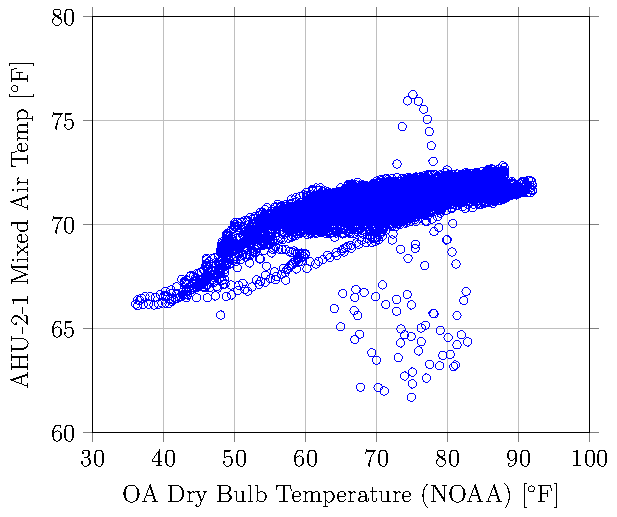
\includegraphics[]{Plots/2016-06-13-1441-AHU21MixedAirTempvsOADryBulbTemperatureNOAA.pdf}
\caption{AHU-2-1 mixed air temperature vs. outdoor air temperature.}
\label{fig:AHU21MixedAirTempvsOADryBulbTemperatureNOAA}
\end{figure}


\begin{figure}
\centering
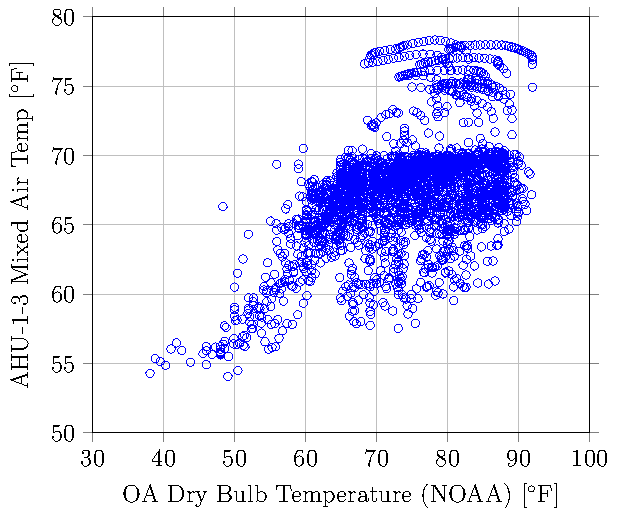
\includegraphics[]{Plots/2016-06-13-1459-AHU13MixedAirTempvsOADryBulbTemperatureNOAA.pdf}
\caption{AHU-1-3 mixed air temperature vs. outdoor air temperature.}
\label{fig:AHU13MixedAirTempvsOADryBulbTemperatureNOAA}
\end{figure}


The result of a \textit{nearest neighbor} approach is shown in \figref{} \ref{fig:AHU13MixedAirTempvsOADryBulbTemperatureNOAA-2}. The algorithm looked back in history (at least a day before) under the following parameters:

\begin{itemize}
    \item The same day of the week
    \item Same hour of day \(\pm\)1 hr.
    \item Same \(\oat{}\) \(\pm\)3\(^\circ\)F
    \item Searching backwards incrementally until 30 data points found
\end{itemize}

The median of the found data points is the resulting prediction. The following
plots show the model fits for the different air handling units at NCTM. The
data covers a period of 180 days. Figures
\ref{fig:2016-09-07-1218-AHU12MixedAirTempvsOADryBulbTemperatureNOAA} and
\ref{fig:AHU13MixedAirTempvsOADryBulbTemperatureNOAA-2} show that the
prediction algorithm can adequately handle the differences from when the air
handling unit is on as well as off. The significant amount of spread in the
mixed air temperature is due to data in which the air handler turns off and is
allowed to drift, typically to a higher temperature in the climate of College
Station. 

Figures
\ref{fig:2016-09-07-1335-MixedAirTempPredictionforContainerAHU12vsAHU12MixedAirTemp}
through
\ref{fig:2016-09-07-1623-MixedAirTempPredictionforContainerAHU23vsAHU23MixedAirTemp}
show the model fits during times when the air handling units are off, ignoring
weekends and holidays, and times between 6:00 PM and 8:00 AM.

\newcommand{\matcaption}[1]{#1 \(\mat\) prediction for data from Mar. 10, 2016 - Sept. 5, 2016, not ignoring any data.}

\begin{figure}
\centering
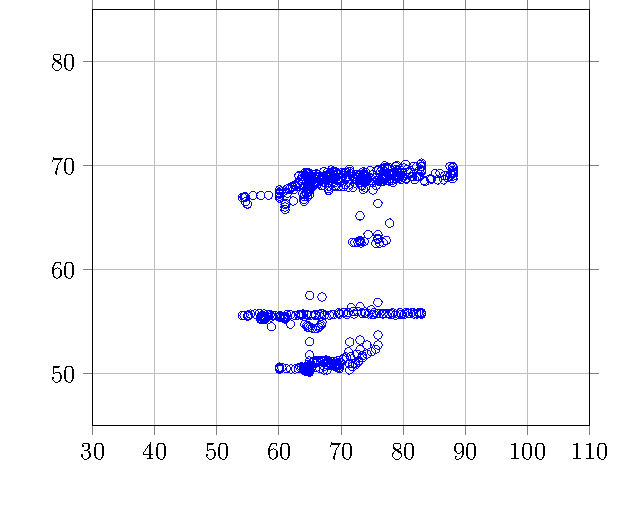
\includegraphics[]{Plots/2016-09-07-1218-AHU12MixedAirTempvsOADryBulbTemperatureNOAA.pdf}
\caption{\matcaption{AHU-1-2}}
\label{fig:2016-09-07-1218-AHU12MixedAirTempvsOADryBulbTemperatureNOAA}
\end{figure}

\begin{figure}
\centering
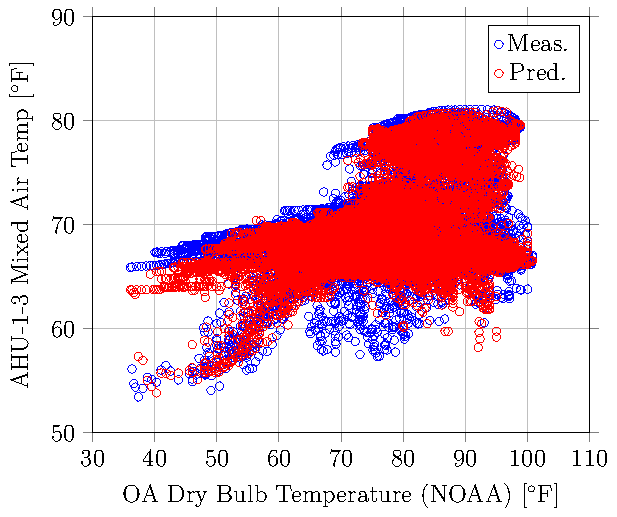
\includegraphics[]{Plots/2016-09-07-0943-AHU13MixedAirTempvsOADryBulbTemperatureNOAA.pdf}
\caption{AHU-1-3 mixed air temperature prediction for data from Mar. 10, 2016 - Sept. 5, 2016, not ignoring any data.}
\label{fig:AHU13MixedAirTempvsOADryBulbTemperatureNOAA-2}
\end{figure}



%% 45 degree plots showing the adequacy of the model fit. 

\newcommand{\mixAirCaptionTwo}[1]{Mixed air temperature prediction results for #1.}

\begin{figure}
\centering
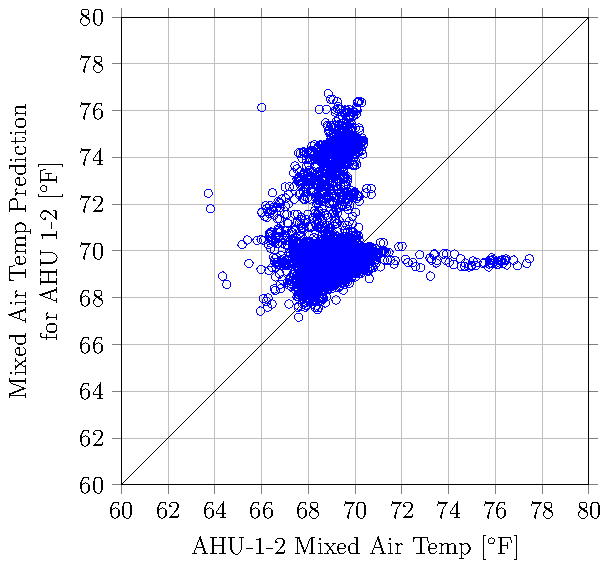
\includegraphics[]{Plots/2016-09-07-1335-MixedAirTempPredictionforContainerAHU12vsAHU12MixedAirTemp.pdf}
\caption{\mixAirCaptionTwo{AHU-1-2}}
\label{fig:2016-09-07-1335-MixedAirTempPredictionforContainerAHU12vsAHU12MixedAirTemp}
\end{figure}

\begin{figure}
\centering
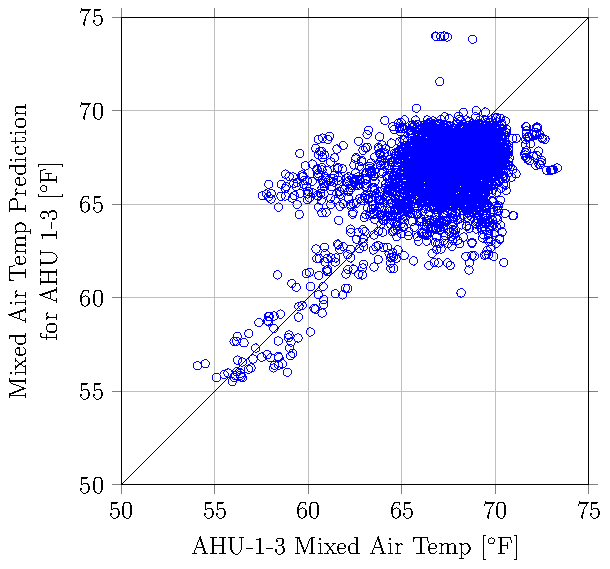
\includegraphics[]{Plots/2016-09-07-1346-MixedAirTempPredictionforContainerAHU13vsAHU13MixedAirTemp.pdf}
\caption{\mixAirCaptionTwo{AHU-1-3}}
\label{fig:2016-09-07-1346-MixedAirTempPredictionforContainerAHU13vsAHU13MixedAirTemp}
\end{figure}

\begin{figure}
\centering
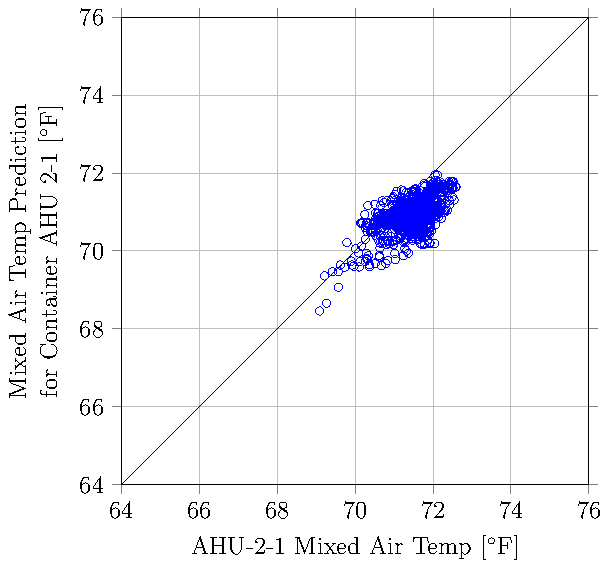
\includegraphics[]{Plots/2016-09-07-1357-MixedAirTempPredictionforContainerAHU21vsAHU21MixedAirTemp.pdf}
\caption{\mixAirCaptionTwo{AHU-2-1}}
\label{fig:2016-09-07-1357-MixedAirTempPredictionforContainerAHU21vsAHU21MixedAirTemp}
\end{figure}

\begin{figure}
\centering
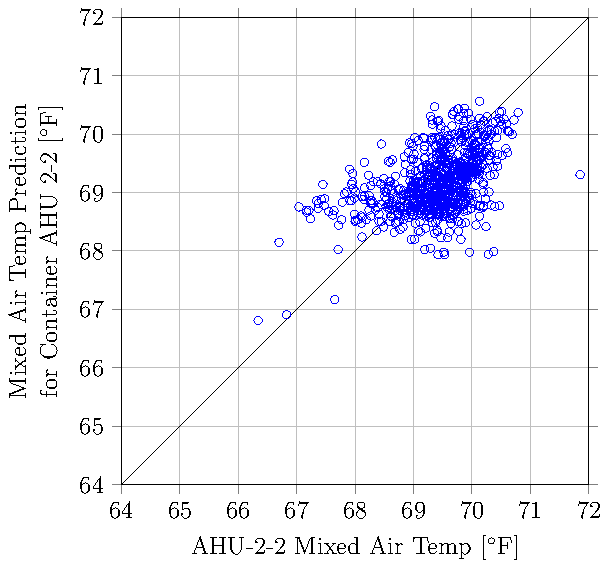
\includegraphics[]{Plots/2016-09-07-1619-MixedAirTempPredictionforContainerAHU22vsAHU22MixedAirTemp.pdf}
\caption{\mixAirCaptionTwo{AHU-2-2}}
\label{fig:2016-09-07-1619-MixedAirTempPredictionforContainerAHU22vsAHU22MixedAirTemp}
\end{figure}

\begin{figure}
\centering
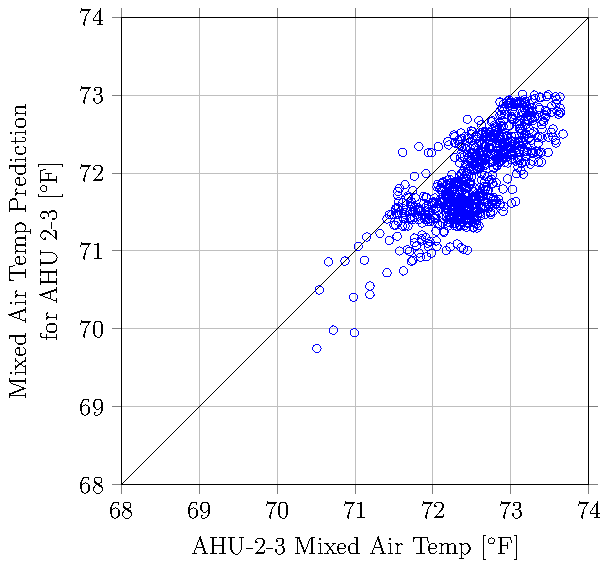
\includegraphics[]{Plots/2016-09-07-1623-MixedAirTempPredictionforContainerAHU23vsAHU23MixedAirTemp.pdf}
\caption{\mixAirCaptionTwo{AHU-2-3}}
\label{fig:2016-09-07-1623-MixedAirTempPredictionforContainerAHU23vsAHU23MixedAirTemp}
\end{figure}


The sensitivity to the ``nearest neighbor'' parameters was tested. The
parameter values were varied as shown in \tableref{}
\ref{tab:NearestNeighborVariations}.

\begin{table}
\centering
\caption{Variations in the parameters for the nearest neighbor algorithm.}
\label{tab:NearestNeighborVariations}
\begin{tabular}{rl}
    Threshold & Variations \\ \midrule
    Time stamp threshold & 15, 30, and 60 minutes \\
    \(T_{oa} \) threshold & \SI{1}{\degF}, \SI{3}{\degF}, \SI{5}{\degF} \\
    Data points threshold & 15, 30, and 45 data points. 
\end{tabular}
\end{table}


With three parameters and 3 different variations for each, this resulted
in 27 test cases. The results from this testing are shown in \tableref{}
\ref{tab:MATTestingResults}. TS stands for time stamps, and is the
number of timestamps threshold. Since the data was on 15 minute
intervals, a 1 timestamp threshold implies a threshold of \(\pm\)15
minutes and a 4 timestamp threshold implies a threshold of \(\pm\)60
minutes. The best model fit used a time stamp threshold of \(\pm\)60
minutes, \(\pm\SI{3}{\degF}\) for \(T_{oa}\), and 15 data points. The
worst case was using \(\pm\)15 minutes, \(\pm \SI{1}{\degF}\), and 30
data points. 

The model was not sensitive to the parameters. The CVs ranged from
1.76\% to 2.16\%. The models with the lowest CVs had the largest range
in the time stamp and \(T_{oa}\) threshold. This is an indication that
using more recent data was more valuable than using data from conditions
matching more closely. 

\begin{table}
    \centering
    \caption{Results from testing different nearest neighbor model
    parameters for predicted \(T_{ma}\).}
    \label{tab:MATTestingResults}
    \begin{tabular}{@{}lllll@{}}
        \toprule
        Run & TS & \(T_{oa}\) & DP & Average CV \\ \midrule
        1   & 1  & 1          & 15 & 2.02\%     \\
        2   & 2  & 1          & 15 & 1.91\%     \\
        3   & 4  & 1          & 15 & 1.80\%     \\
        4   & 1  & 3          & 15 & 1.90\%     \\
        5   & 2  & 3          & 15 & 1.84\%     \\
        6   & 4  & 3          & 15 & 1.76\%     \\
        7   & 1  & 5          & 15 & 1.82\%     \\
        8   & 2  & 5          & 15 & 1.80\%     \\
        9   & 4  & 5          & 15 & 1.77\%     \\
        10  & 1  & 1          & 30 & 2.13\%     \\
        11  & 2  & 1          & 30 & 2.01\%     \\
        12  & 4  & 1          & 30 & 1.85\%     \\
        13  & 1  & 3          & 30 & 1.98\%     \\
        14  & 2  & 3          & 30 & 1.90\%     \\
        15  & 4  & 3          & 30 & 1.79\%     \\
        16  & 1  & 5          & 30 & 1.90\%     \\
        17  & 2  & 5          & 30 & 1.82\%     \\
        18  & 4  & 5          & 30 & 1.77\%     \\
        19  & 1  & 1          & 45 & 2.16\%     \\
        20  & 2  & 1          & 45 & 2.10\%     \\
        21  & 4  & 1          & 45 & 1.93\%     \\
        22  & 1  & 3          & 45 & 2.00\%     \\
        23  & 2  & 3          & 45 & 1.99\%     \\
        24  & 4  & 3          & 45 & 1.83\%     \\
        25  & 1  & 5          & 45 & 1.92\%     \\
        26  & 2  & 5          & 45 & 1.88\%     \\
        27  & 4  & 5          & 45 & 1.78\%     \\ \bottomrule
    \end{tabular}
\end{table}

\sisetup{round-mode=figures, round-precision=3}

\begin{table}
\centering
\caption{\(T_{ma}\) prediction results using the parameters in Run 6.}
\label{tab:MATPredictionResultsForRun6}
\begin{tabular}{lS} \toprule
    AHU     & {RMSE (\si{\degF})  } \\ \midrule
    AHU 1-2 & \num{1.686834982}   \\
    AHU 1-3 & \num{2.41776849}    \\
    AHU 1-4 & \num{1.251856851}   \\
    AHU 2-1 & \num{0.744179046}   \\
    AHU 2-2 & \num{0.619408965}   \\
    AHU 2-3 & \num{0.495786538}   \\ \bottomrule
\end{tabular}
\end{table}

\section{Analysis of the Plenum Air Temperature}

Under certain assumptions, the plenum air temperature for the series fan
powered terminal units is possible. If the terminal unit is modeled as a simple
mixing problem, the plenum air temperature will be 
\begin{equation}
    T_{plenum}=\frac{\flow{tot}T_{dis}-\flow{pri}T_{sa}}{\flow{tot} -\flow{pri}}
\end{equation}

Since \(T_{plenum}\) is a function of 4 variables, it is important to
consider the uncertainty in the estimation. Clearly, when
\(\flow{plenum}\) is low, assumed to be equivalent to \(\flow{tot} -
\flow{pri}\), the uncertainty in  \(T_{plenum}\) grows significantly and
when the flow is equal to zero \(T_{plenum}\) is undefined. 

Using the Kline-McKlintock formulation of uncertainty, the uncertainty
of \(T_{plenum}\) is 

\begin{multline}
    \delta T_{plen} = \left[\left( \pdv{T_{plen}}{\flow{pri}} \delta \flow{pri}   \right)^2  +\left( \pdv{T_{plen}}{\flow{tot}} \delta \flow{tot}   \right)^2 + \right. \\
    \left. \left( \pdv{T_{plen}}{T_{dis}} \delta T_{dis}   \right)^2 + \left( \pdv{T_{plen}}{T_{sa}} \delta T_{sa}   \right)^2  \right]^{1/2}
\end{multline}

\begin{multline}\label{eq:plenumUncertainty}
    \delta T_{plen} = \left[\left(  \frac{\flow{tot}\left(T_{dis}-T_{sa} \right)}{{\flow{plen}}^2}   \delta \flow{pri} \right)^2  +\left(\frac{\flow{pri}\left(T_{sa}-T_{dis} \right)}{{\flow{plen}}^2}      \delta \flow{tot}   \right)^2 + \right. \\
    \left. \left( \frac{\flow{tot}}{\flow{plen}} \delta T_{dis}   \right)^2 + \left(\frac{\flow{pri}}{\flow{plen}}  \delta T_{sa}   \right)^2  \right]^{1/2}
\end{multline}

So for an example if, 

\newcommand{\flowtotvalue}{\SI{2200}{\CFM}}
\newcommand{\plenflowvalue}{\SI{1000}{\CFM}}

\begin{itemize}
    \item \(\totflow{}=\flowtotvalue\)
    \item \(\plenflow{}=\plenflowvalue\)
    \item \(\priflow=\flowtotvalue - \plenflowvalue = \SI{1200}{\CFM} \)
    \item \(\sat = 55^{\circ}\text{F} \)
    \item \(\dat = 75^{\circ}\text{F} \)
    \item \(\delta\priflow{}=\delta\plenflow=\delta\totflow=100 \text{ CFM}\)
    \item \(\delta \sat = \delta \dat = 1^{\circ} \text{F} \)
\end{itemize}

Equation \ref{eq:plenumUncertainty} becomes
\begin{equation}\label{eq:plenumUncertainty2}
    \delta T_{plen} = \left[\left(  \SI{3.06}{\degreeF}  \right)^2  +\left( \SI{-1.39}{\degreeF}  \right)^2 +  \left( \SI{1.83}{\degreeF} \right)^2 + \left(\SI{0.83}{\degreeF}  \right)^2  \right]^{1/2}
\end{equation}
which results in a final uncertainty of \SI{3.91}{\degreeF}.

As an example as to how unstable the calculation for the plenum
temperature is, \figref{}
\ref{fig:2016-09-16-1006-PlenumTemperatureforContainerFPVAV19vsZoneLoadforContainerFPVAV19}
shows the calculation for FPVAV-1-9 over the period from February 1,
2016 - May 1, 2016. The calculated values are unrealistic ranging from
-1,500\(^\circ\)F to 1,500\(^\circ\)F. The reason for this is made clear
in a time series plots of the flows related to the terminal unit. As
shown in \figref{} \ref{fig:2016-09-16-1639-FPVAV19AIRVOLUME-TikzData},
for this particular terminal unit, the primary flow is either near zero
or design. At times, the measured flow is also above the design
spec, making the plenum flow calculation zero. When the plenum flow is
calculated to be zero, the plenum temperature calculation becomes
undefined.

Using the assumptions that the uncertainty in the flow was 100 CFM and
the uncertainty in the temperature measurements was 1\(^\circ\)F, the
plenum temperature was recorded and plotted versus \(\oat\) from October
6, 2015 to September 12, 2016, ignoring items that appear in \tableref{}
\ref{tab:PlenumTemperatureEstimation}. The distribution statistics for
each terminal unit is found in \tableref{} \ref{tab:plenumStatistics}.
The table is listed in ascending order by the median of the plenum
temperature calculated.

To notice is that percentage of ignored points is below 96\% for only 4
terminal units.  The majority of the points are ignored because the
uncertainty in the calculation is above the 2\(^\circ\)F threshold that
was arbitrarily chosen.  In fact, at no point was the uncertainty below
2\(^\circ\)F for FPVAV-2-7.  The median plenum temperature ranges from
58.8\(^\circ\)F for FPVAV-1-8 to 75.6\(^\circ\)F for FPVAV-1-6.

Another interesting way to examine the difference between the plenum
temperature and the zone temperature is to plot the estimated reheat in
the terminal unit when the reheat valve is closed.  Ideally, the amount
of reheat would be at or near zero. 

If the plenum temperature is assumed to be equal to the zone temperature
then an estimate of the mixed air temperature in the terminal unit would
be
\begin{equation}
    \mat = \frac{\priflow \sat + T_{zone} \left( \totflow - \priflow \right) }{ \totflow}
    \label{eq:TerminalUnitMixedAirTemp}
\end{equation}
and the reheat energy could be estimated by
\begin{equation}
    \heatenergy = 1.08 \left( CFM \right) \left( \mat - \dat  \right)
    \label{eq:TerminalUnitReheatEnergy}
\end{equation}

\figref{}s
\ref{fig:2016-10-19-1424-ZoneReheatEnergyforContainerFPVAV216vsOADryBulbTemperatureNOAA}
through
\ref{fig:2016-10-19-1521-ZoneReheatEnergyforContainerFPVAV213vsOADryBulbTemperatureNOAA}
show the reheat energy as determined by \eqreftext{}
\ref{eq:TerminalUnitReheatEnergy}. They are from the period of February
1, 2016 through May 1, 2016.  Timestamps during weekends, times between
5:00 PM and 9:00 AM, and when the corresponding reheat valve command is
\( < 1 \) were ignored. Again, ideally, the reheat value would be
exactly zero.


\begin{table}
\centering
\caption{Implementer settings for plenum temperature estimation for NCTM, used to calculate data in \tableref{} \ref{tab:plenumStatistics}.}
\label{tab:PlenumTemperatureEstimation}
\begin{tabular}{@{}rl@{}}
\toprule
Project:            & Mitch Dissertation NCTM---2016-09-19 10:34           \\ \midrule
Scope:              & NCTM                                                 \\
Axis Parameters:    & Plenum Temperature vs. OA Dry-bulb Temp (NOAA)       \\
Date Period:        & 10/6/2015 - 9/12/2016  (342 days)                    \\
OAT range:          & 31 to 100\(^\circ\)F                                 \\
Ignoring:           & When AHU is Off                                      \\
                    & First 1.0 hours of operation                         \\
                    & Last 1.0 hours of operation                          \\
                    & Sundays                                              \\
                    & Saturdays                                            \\
                    & Federal Holidays                                     \\
                    & Hours from 17:00 to 9:00                             \\
                    & When label Plenum Temp Uncertainty is greater than 2 \\
                    & When label Valve Positions is greater than 1         \\ \bottomrule
\end{tabular}
\end{table}



\begin{figure}
\centering

\includegraphics[]{Plots/2016-09-16-1006-PlenumTemperatureforContainerFPVAV19vsZoneLoadforContainerFPVAV19.pdf}
\caption{Calculated plenum temperature for FPVAV-1-9.}
\label{fig:2016-09-16-1006-PlenumTemperatureforContainerFPVAV19vsZoneLoadforContainerFPVAV19}
\end{figure}

\begin{figure}
\centering
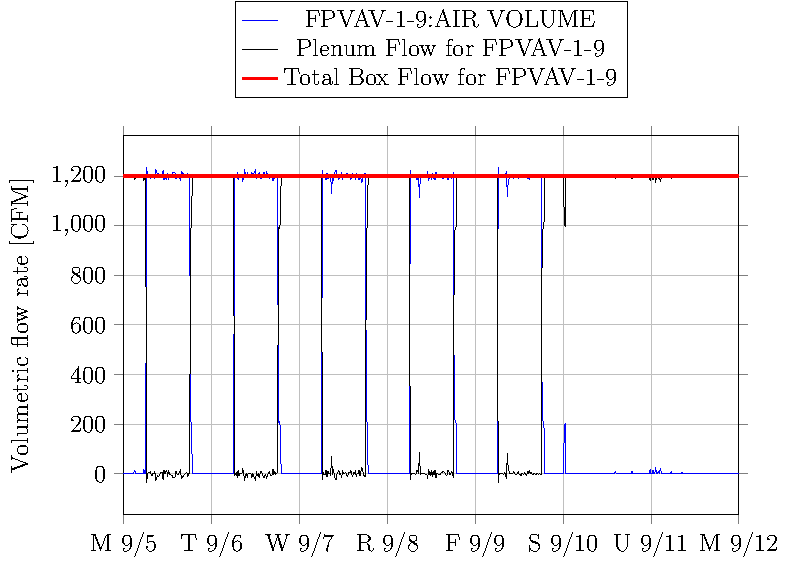
\includegraphics[]{Plots/2016-09-16-1639-FPVAV19AIRVOLUME-TikzData.pdf}
\caption{Flowrates for FPVAV-1-9}
\label{fig:2016-09-16-1639-FPVAV19AIRVOLUME-TikzData}
\end{figure}

\begin{table}
\centering
\caption{Calculated plenum temperature statistics for NCTM.}
\label{tab:plenumStatistics}
\begin{tabular}{@{}llllllllll@{}}
    \toprule
Unit     & Min  & \parbox{1cm}{5th \\ Perc.} & Mean & Median & \parbox{1cm}{95th \\ Perc.} & Max   & \parbox{1cm}{St. \\ Dev. }      & \parbox{1cm}{Original \\ Count} & \parbox{1 cm}{\% \\ Ignored } \\ \midrule
1-8  & 56.5 & 56.5 & 60.6 & 58.8 & 71.8 & 71.8 & 4.25 & \num{29199} & 99.911\%         \\
2-12 & 52.8 & 55.7 & 60.8 & 61.8 & 62.5 & 75.0 & 2.23 & \num{29319} & 88.062\%         \\
2-15 & 52.1 & 57.4 & 61.3 & 61.8 & 62.6 & 78.5 & 1.84 & \num{29324} & 78.645\%         \\
1-9  & 57.0 & 57.0 & 63.6 & 65.0 & 73.5 & 73.8 & 5.34 & \num{27961} & 99.939\%         \\
2-6  & 65.0 & 65.0 & 65.0 & 65.0 & 65.0 & 65.0 & 0.00 & \num{29311} & 99.997\%         \\
2-18 & 61.5 & 62.7 & 69.6 & 67.0 & 80.2 & 80.5 & 5.60 & \num{29312} & 99.846\%         \\
2-16 & 67.0 & 67.0 & 67.3 & 67.5 & 67.5 & 67.5 & 0.29 & \num{29325} & 99.990\%         \\
2-10 & 66.5 & 66.5 & 67.8 & 67.8 & 69.0 & 69.0 & 1.44 & \num{29236} & 99.986\%         \\
2-14 & 60.0 & 61.0 & 68.8 & 68.5 & 79.0 & 79.8 & 6.28 & \num{29318} & 99.860\%         \\
2-11 & 66.5 & 66.5 & 68.0 & 68.5 & 69.5 & 69.5 & 1.01 & \num{28557} & 99.958\%         \\
2-5  & 68.5 & 68.5 & 69.1 & 69.0 & 70.0 & 70.0 & 0.65 & \num{29309} & 99.983\%         \\
2-8  & 68.2 & 69.1 & 70.0 & 70.0 & 70.7 & 72.5 & 0.55 & \num{29304} & 98.601\%         \\
2-13 & 68.0 & 68.5 & 70.0 & 70.0 & 71.5 & 72.6 & 1.34 & \num{29312} & 99.887\%         \\
1-5  & 55.0 & 63.8 & 71.1 & 70.1 & 78.0 & 79.0 & 4.62 & \num{30170} & 99.450\%         \\
2-17 & 61.5 & 68.5 & 70.3 & 70.4 & 71.5 & 72.5 & 1.23 & \num{29287} & 99.126\%         \\
2-2  & 52.5 & 67.3 & 70.7 & 70.8 & 73.6 & 75.6 & 2.69 & \num{29363} & 98.685\%         \\
1-7  & 60.0 & 64.5 & 71.8 & 71.8 & 75.1 & 75.7 & 3.11 & \num{29955} & 99.222\%         \\
2-3  & 64.5 & 71.0 & 73.0 & 72.8 & 75.3 & 76.2 & 1.49 & \num{29367} & 96.391\%         \\
1-2  & 67.0 & 70.8 & 73.9 & 72.9 & 77.8 & 78.5 & 2.60 & \num{30166} & 99.589\%         \\
2-1  & 67.5 & 70.8 & 73.6 & 73.8 & 75.5 & 81.7 & 1.44 & \num{29366} & 96.016\%         \\
1-3  & 71.4 & 72.6 & 74.2 & 74.4 & 75.4 & 76.9 & 0.94 & \num{30145} & 98.202\%         \\
2-9  & 69.0 & 70.7 & 73.9 & 74.5 & 76.5 & 78.4 & 1.88 & \num{29272} & 76.356\%         \\
1-1  & 57.0 & 71.8 & 74.6 & 74.8 & 79.0 & 82.5 & 2.64 & \num{30152} & 97.652\%         \\
1-10 & 58.5 & 62.0 & 73.8 & 74.9 & 76.0 & 78.2 & 3.61 & \num{29941} & 99.008\%         \\
1-4  & 54.0 & 72.4 & 74.9 & 75.1 & 77.2 & 81.7 & 2.51 & \num{30086} & 98.488\%         \\
2-4  & 69.5 & 73.7 & 75.3 & 75.2 & 76.7 & 77.6 & 0.96 & \num{29304} & 86.916\%         \\
1-6  & 56.5 & 66.2 & 74.1 & 75.6 & 81.3 & 81.6 & 5.43 & \num{30170} & 99.738\%         \\
2-7  & N/A  & N/A  & N/A  & N/A  & N/A  & N/A  & N/A  & \num{28906} & 100.000\%        \\ \bottomrule
\end{tabular}
\end{table}

% For series fan powered terminal units, the assumption was made that the total
% flow remains constant and that the mixed air temperature at the
% individual terminal unit can be predicted based on the primary flow value that is
% measured. 

% One possible assumption for the plenum temperature is that it is equal to the
% corresponding zone temperature. An interesting analysis is then to calculate
% the mixed air temperature based on this assumption and then look at times when
% the reheat valve is commanded to zero. It would be expected that the calculated
% reheat would be near zero, if not slightly above zero due to leakage in the
% reheat valve.  The next series of plots look at data from February 1, 2016 to
% May 1, 2016, ignoring when the unit is off, weekends and holidays, and when the
% commanded reheat coil position is greater than 1\%. 

\figref{}
\ref{fig:2016-10-19-1424-ZoneReheatEnergyforContainerFPVAV216vsOADryBulbTemperatureNOAA}
shows an example of where the assumption appears to hold properly.  The
vast majority of the points are greater than \SI{0}{\BTU\per\hour}.

\figref{}
\ref{fig:2016-10-19-1438-ZoneReheatEnergyforContainerFPVAV24vsOADryBulbTemperatureNOAA}
shows a case in which there is either constant reheat or the actual
plenum temperature is lower than the zone temperature that was assumed.

\figref{}
\ref{fig:2016-10-19-1521-ZoneReheatEnergyforContainerFPVAV213vsOADryBulbTemperatureNOAA}
shows a case in which the reheat is estimated to be a negative value,
which likely means that the actual plenum temperature is greater than
the assumed plenum temperature equal to the zone temperature. 

\begin{figure}
\centering
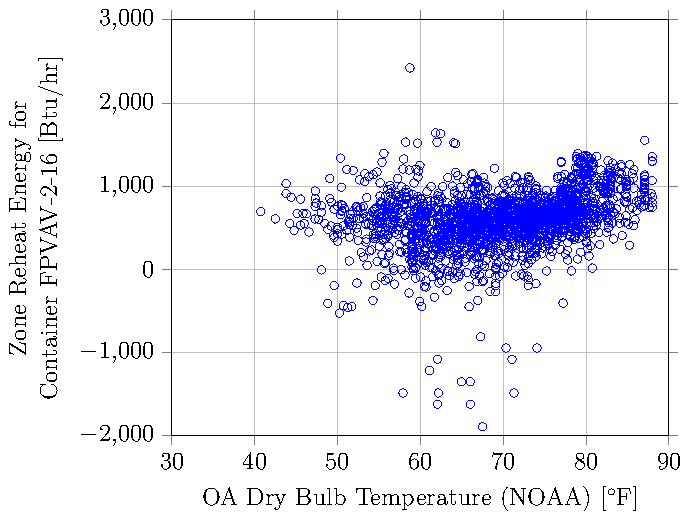
\includegraphics[]{Plots/2016-10-19-1424-ZoneReheatEnergyforContainerFPVAV216vsOADryBulbTemperatureNOAA.pdf}
\caption{Zone reheat energy for terminal unit 2-16.}
\label{fig:2016-10-19-1424-ZoneReheatEnergyforContainerFPVAV216vsOADryBulbTemperatureNOAA}
\end{figure}

\begin{figure}
\centering
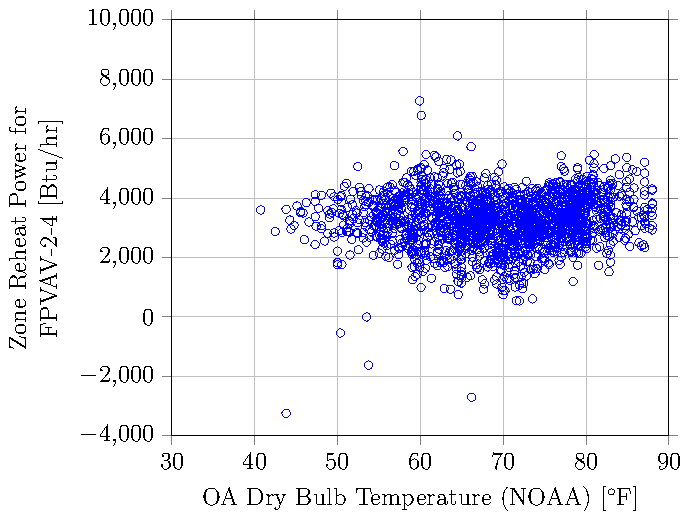
\includegraphics[]{Plots/2016-10-19-1438-ZoneReheatEnergyforContainerFPVAV24vsOADryBulbTemperatureNOAA.pdf}
\caption{Zone reheat energy for terminal unit 2-4.}
\label{fig:2016-10-19-1438-ZoneReheatEnergyforContainerFPVAV24vsOADryBulbTemperatureNOAA}
\end{figure}

\begin{figure}
\centering
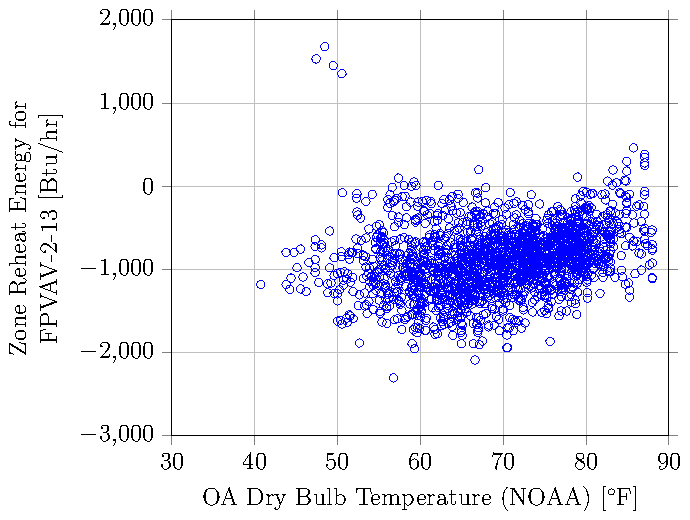
\includegraphics[]{Plots/2016-10-19-1521-ZoneReheatEnergyforContainerFPVAV213vsOADryBulbTemperatureNOAA.pdf}
\caption{Zone reheat energy for terminal unit 2-13.}
\label{fig:2016-10-19-1521-ZoneReheatEnergyforContainerFPVAV213vsOADryBulbTemperatureNOAA}
\end{figure}

Another way to view the accuracy and importance of the plenum
temperature on the amount of reheat necessary is to look at the
difference between the discharge temperature and the predicted mixed air
temperature in the terminal unit under conditions when the reheat valve
is closed.  During these times the values should be nearly equal, and the
difference should be near zero. 

Under the assumption that the plenum temperature is equal to the
corresponding zone temperature, it does not appear as if this assumption
is valid for corresponding energy calculations. \figref{}
\ref{fig:2017-01-09-1412-TboxDischargeMixedAirTempfromRoomTempforFPVAV27vsTboxPLRforFPVAV27}
shows as much as an \SI{8}{\degreeF} difference. Because the value is
positive, this means that the plenum temperature is likely higher than
the assumed zone temperature, assuming that the measured discharge
temperature is more accurate that the estimation of the plenum
temperature. 

\begin{figure}
\centering
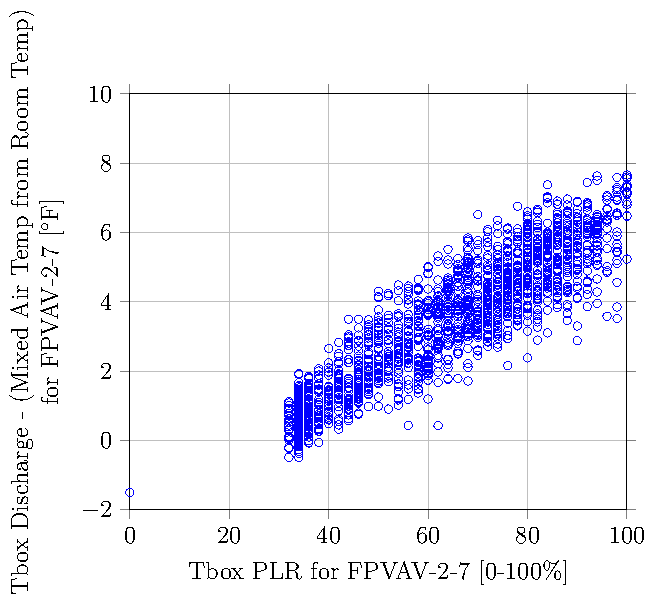
\includegraphics[]{Plots/2017-01-09-1412-TboxDischargeMixedAirTempfromRoomTempforFPVAV27vsTboxPLRforFPVAV27.pdf}
\caption{Difference between discharge temperature and predicted mixed
air temperature using the zone temperature assumption for TU-2-7.}
\label{fig:2017-01-09-1412-TboxDischargeMixedAirTempfromRoomTempforFPVAV27vsTboxPLRforFPVAV27}
\end{figure}

The opposite case can be seen with TU-2-15, as shown in \figref{}
\ref{fig:2017-01-09-1434-TboxDischargeMixedAirTempfromRoomTempforFPVAV215vsTboxPLRforFPVAV215}
In this case, the values are all negative, indicating that the plenum
temperature is lower than the zone temperature. The plots are from the
same period and cover a wide range of outdoor air temperatures from
\SI{36}{\degreeF} to \SI{96}{\degreeF}. Both plots do appear linear with
regards to the PLR of the terminal unit. This linearity indicates that there is
some relationship with the plenum temperature and the amount of
conditioned air coming from the parent air handling unit.

\begin{figure}
\centering
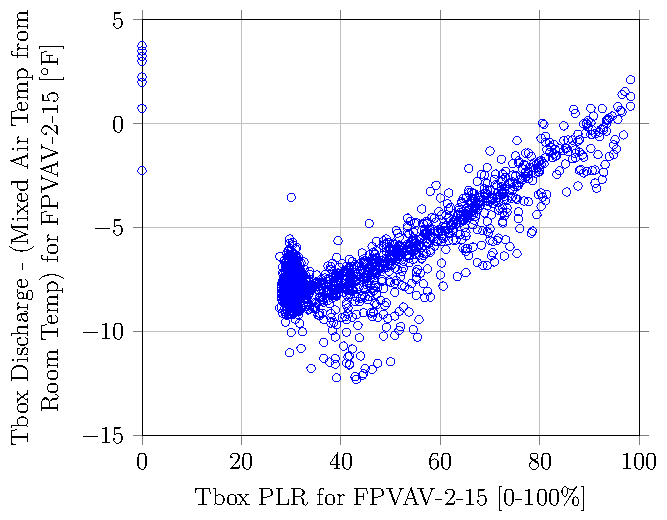
\includegraphics[]{Plots/2017-01-09-1434-TboxDischargeMixedAirTempfromRoomTempforFPVAV215vsTboxPLRforFPVAV215.pdf}
\caption{Difference between discharge temperature and predicted mixed
air temperature using the zone temperature assumption for TU-2-15.}
\label{fig:2017-01-09-1434-TboxDischargeMixedAirTempfromRoomTempforFPVAV215vsTboxPLRforFPVAV215}
\end{figure}


This linear dependence on the PLR does not carry to all the terminal
units. As a counterexample to the previous plots, FPVAV-2-10 has a
zig-zag pattern. 


\begin{figure}
\centering
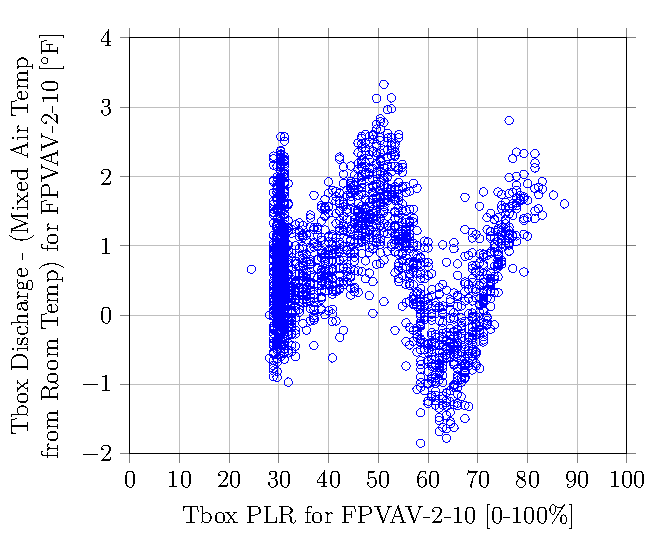
\includegraphics[]{Plots/2017-01-10-0906-TboxDischargeMixedAirTempfromRoomTempforFPVAV210vsTboxPLRforFPVAV210.pdf}
\caption{Difference between discharge temperature and predicted mixed
air temperature using the zone temperature assumption for FPVAV-2-10.}
\label{fig:2017-01-10-0906-TboxDischargeMixedAirTempfromRoomTempforFPVAV210vsTboxPLRforFPVAV210}
\end{figure}




\section{Analysis of Zone Load Predictions}

An important factor in the optimization methodology is the prediction of
the zone loads at a given time, without access to current live sensor
information. 

Before analyzing the prediction ability of different zone loads, it is
important to gather insight into the nature of the calculated variable
that is proposed to be used as the surrogate for zone load.   

If the zone loads are being met and steady-state conditions are assumed,
the sensible zone load will be
\begin{equation}
    Q_{zone}=\flow{z} \rhocp{} \left(T_{dis}-T_{z} \right) \approx 1.08 \cdot \flow{z}\left(T_{dis}-T_{z} \right)
\end{equation}

As a result of the dynamics of how terminal units are controlled in reality,
the estimated zone load can vary back and forth, while the true zone load is a
more smooth function. \figref{}
\ref{fig:2016-06-22-1654-ZoneLoadforContainerFPVAV17-TikzData} shows how the
estimated zone load can change directionality several times over the course of
a day. The zone load for terminal unit FPVAV-1-7 typically varied from 6,000
BTU/hr to 20,000 BTU/hr over the course of the week from June 6, 2016, to June
11, 2016.

\figref{} \ref{fig:2016-06-22-1643-ZoneLoadforContainerFPVAV22-TikzData}
shows another example of how the estimated zone load may vary throughout
a typical week. \figref{}
\ref{fig:2016-06-22-1643-ZoneLoadforContainerFPVAV22-TikzData} shows the
zone load for FPVAV-2-2, which experiences a significant load compared
to the other terminal units at NCTM. The zone load varies from near
10,000 BTU/hr to near 50,000 BTU/hr at its peak.

With \figref{}
\ref{fig:2016-06-22-1654-ZoneLoadforContainerFPVAV17-TikzData} as
evidence, it is clear that the ``true'' zone load cannot be reasonably
estimated with the trend data that is available in typical BAS systems.
However, the ratio of magnitudes of the load from zone to zone can still
be inferred and be useful in improving the energy efficiency of the
system.  

\begin{figure}
\centering
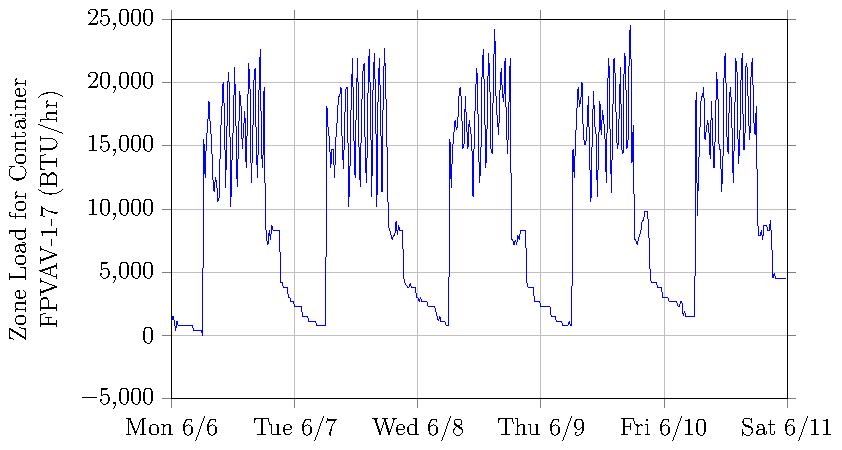
\includegraphics[]{Plots/2016-06-22-1654-ZoneLoadforContainerFPVAV17-TikzData.pdf}
\caption{Zone load estimation for FPVAV-1-7.}
\label{fig:2016-06-22-1654-ZoneLoadforContainerFPVAV17-TikzData}
\end{figure}

\begin{figure}
\centering
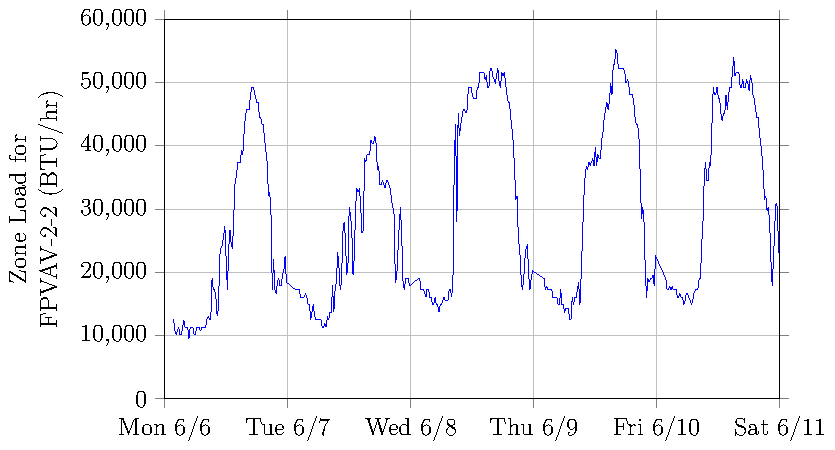
\includegraphics[]{Plots/2016-06-22-1643-ZoneLoadforContainerFPVAV22-TikzData.pdf}
\caption{Zone load estimation for FPVAV-2-2.}
\label{fig:2016-06-22-1643-ZoneLoadforContainerFPVAV22-TikzData}
\end{figure}



\figref{}
\ref{fig:ZoneLoadforContainerFPVAV214vsOADryBulbTemperatureNOAA} shows
an example of the zone load plotted against outdoor air dry-bulb
temperature. Notice that the load is not a well-defined function of
\(\oat\). This turns out to be the case for many of the internal zones,
which have a higher dependence on the time of day parameters. 

\figref{}
\ref{fig:ZoneLoadforContainerFPVAV29vsOADryBulbTemperatureNOAA} shows
the zone load for FPVAV-2-9 versus \(\oat\). FPVAV-2-9 serves only
internal zones, and the load only ranges from approximately 250 BTU/hr
to 4,000 BTU/hr.


\begin{figure}
\centering
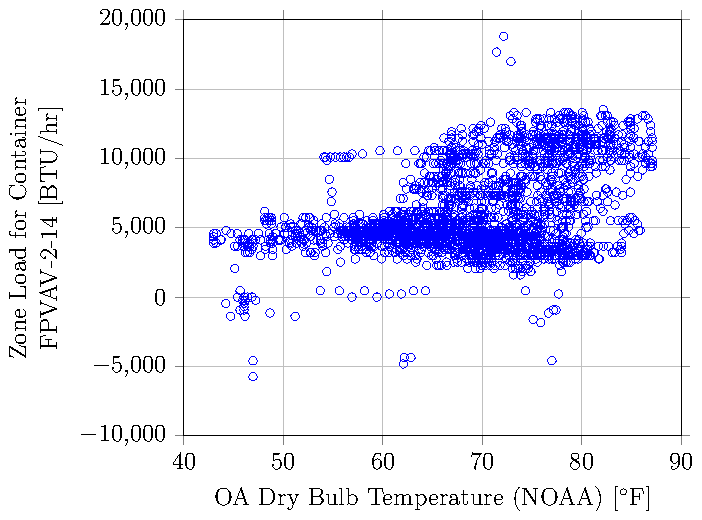
\includegraphics[]{Plots/2016-06-22-1704-ZoneLoadforContainerFPVAV214vsOADryBulbTemperatureNOAA.pdf}
\caption{Calculated zone load for FPVAV-2-14 during the month of April 2016.}
\label{fig:ZoneLoadforContainerFPVAV214vsOADryBulbTemperatureNOAA}
\end{figure}


\begin{figure}
\centering
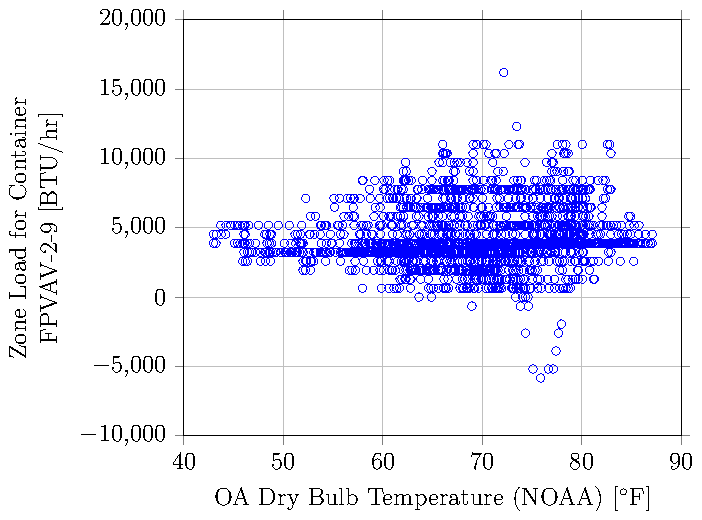
\includegraphics[]{Plots/2016-06-22-1716-ZoneLoadforContainerFPVAV29vsOADryBulbTemperatureNOAA.pdf}
\caption{Calculated zone load for FPVAV-2-9, which serves only internal space, during the month of April 2016.}
\label{fig:ZoneLoadforContainerFPVAV29vsOADryBulbTemperatureNOAA}
\end{figure}


The statistics related to the predictions of the zone loads for data ranging from October 6, 2015 to June 1, 2016 is given in \tableref{} \ref{tab:zoneLoadStats}.


%%Data from NCTM Report 2016-06-20 T 12-16.xlsx.
\begin{table}
\centering
\caption{Statistics related to the prediction of the zone loads at NCTM.}
\small
\label{tab:zoneLoadStats}
\begin{tabular}{lrrrr} 
    \toprule
    Terminal Unit & \parbox{2.3cm}{Med. Abs. \\ \(\epsilon\) (BTU/hr)} & \parbox{2.3cm}{Mean Abs. \\ \(\epsilon\)  (BTU/hr)} &  \parbox{2cm}{RMSE \\ (BTU/hr)} & \parbox{2cm}{MBE \\ (BTU/hr)} \\
    \midrule
FPVAV-2-7  & 108   & 171   & 298    & -41    \\
FPVAV-2-16 & 135   & 385   & 704    & 59     \\
FPVAV-2-5  & 162   & 221   & 328    & -22    \\
FPVAV-2-12 & 203   & 1,058 & 1,885  & -896   \\
FPVAV-2-6  & 216   & 488   & 836    & 24     \\
FPVAV-2-13 & 270   & 784   & 1,841  & 68     \\
FPVAV-2-10 & 292   & 631   & 1,000  & -87    \\
FPVAV-2-11 & 302   & 708   & 1,062  & -68    \\
FPVAV-2-18 & 324   & 914   & 1,614  & 77     \\
FPVAV-1-11 & 324   & 703   & 1,585  & 115    \\
FPVAV-2-14 & 459   & 1,004 & 1,780  & -9     \\
FPVAV-2-4  & 540   & 1,036 & 2,012  & 84     \\
FPVAV-1-2  & 626   & 1,201 & 2,056  & -385   \\
FPVAV-2-8  & 648   & 991   & 1,519  & -43    \\
FPVAV-2-9  & 648   & 1,236 & 1,763  & 635    \\
FPVAV-2-17 & 691   & 1,386 & 2,327  & 122    \\
FPVAV-2-15 & 756   & 3,852 & 12,353 & 552    \\
FPVAV-1-8  & 945   & 1,371 & 1,978  & 336    \\
FPVAV-2-3  & 972   & 1,789 & 3,587  & -171   \\
FPVAV-2-1  & 1,080 & 1,609 & 2,871  & -559   \\
FPVAV-1-9  & 1,296 & 1,850 & 2,805  & 209    \\
FPVAV-1-5  & 1,404 & 2,463 & 4,105  & -17    \\
FPVAV-1-10 & 1,512 & 2,819 & 4,634  & 1,054  \\
FPVAV-1-1  & 1,598 & 3,783 & 6,267  & -1,359 \\
FPVAV-1-3  & 1,755 & 3,164 & 4,868  & -237   \\
FPVAV-1-6  & 1,814 & 3,186 & 4,861  & 261    \\
FPVAV-1-7  & 2,268 & 2,827 & 3,942  & -326   \\
FPVAV-2-2  & 2,376 & 4,422 & 7,184  & 1,773  \\
FPVAV-1-4  & 3,024 & 5,569 & 8,502  & 19     \\
    \bottomrule
\end{tabular}
\end{table}

The highest errors in the prediction were for FPVAV-1-4, the zone that
has the highest overall zone load in the building, by a significant
margin. It has estimated loads near 50,000 BTU/hr.


%% These items come from the analysis done with plus minus 15 min and 3 degree F OAT bounds in file Batch Plots -- Mitch Dissertation N -- 2016-09-14 0952

An interesting pattern that was that the initial prediction routine
overpredicted the zone load when the zone load was closer to the heating
range and underpredicted the zone load during times of high cooling
load. This bias was seen in every terminal unit in the building and this
bias occured with both the largest and smallest terminal units. Figures
\ref{fig:2016-09-14-1028-ZoneLoadResidualforContainerFPVAV22vsZoneLoadforContainerFPVAV22}
through
\ref{fig:2016-09-14-1020-ZoneLoadResidualforContainerFPVAV27vsZoneLoadforContainerFPVAV27}
show examples of this phenomenon. This is due to the fact that the
median of sub-sets of data was used for the prediction. The method will
always underpredict the highest value and overpredict the lowest value.
The date period analyzed was from March 1, 2016 to August 1, 2016,
ignoring when the AHUs were off, federal holidays and weekends, and
hours from 5 PM to 9 AM. 

\newcommand{\zoneLoadCaption}[1]{Bias in zone load prediction for #1.}


\begin{figure}
\centering
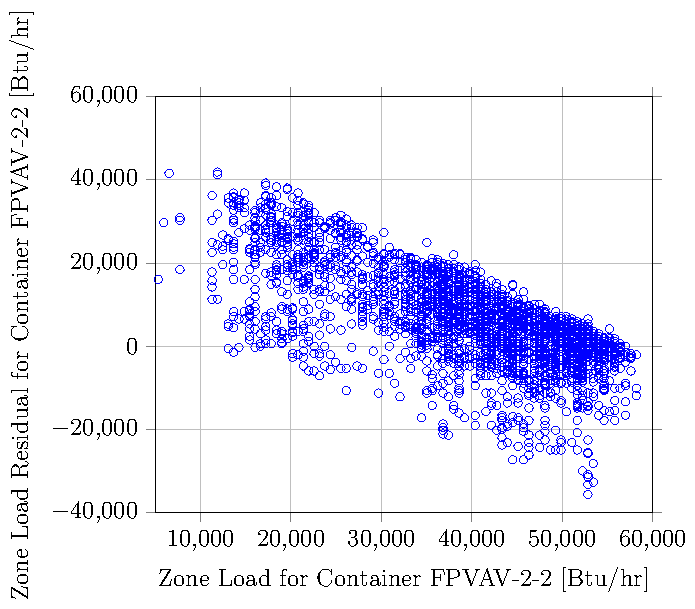
\includegraphics[]{Plots/2016-09-14-1028-ZoneLoadResidualforContainerFPVAV22vsZoneLoadforContainerFPVAV22.pdf}
\caption{\zoneLoadCaption{FPVAV-2-2}}
\label{fig:2016-09-14-1028-ZoneLoadResidualforContainerFPVAV22vsZoneLoadforContainerFPVAV22}
\end{figure}

\begin{figure}
\centering
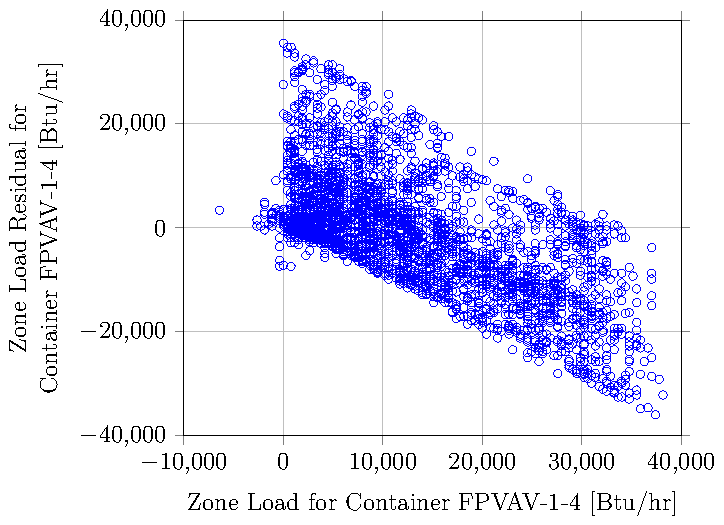
\includegraphics[]{Plots/2016-09-14-1007-ZoneLoadResidualforContainerFPVAV14vsZoneLoadforContainerFPVAV14.pdf}
\caption{\zoneLoadCaption{FPVAV-1-4}}
\label{fig:2016-09-14-1007-ZoneLoadResidualforContainerFPVAV14vsZoneLoadforContainerFPVAV14}
\end{figure}

\begin{figure}
\centering
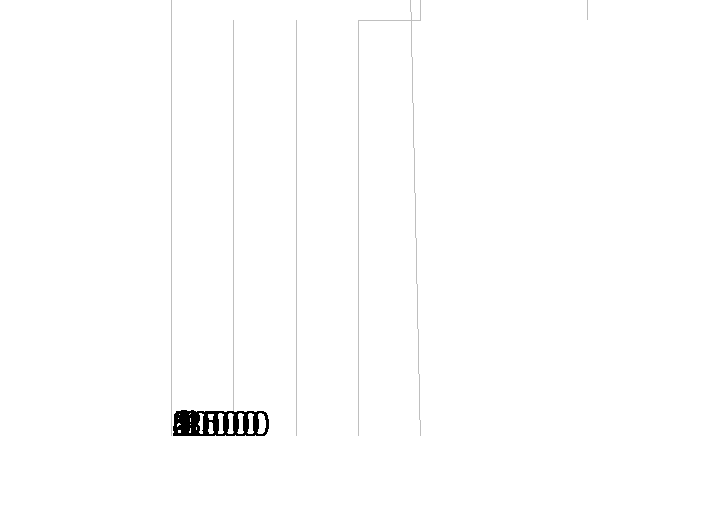
\includegraphics[]{Plots/2016-09-14-1020-ZoneLoadResidualforContainerFPVAV27vsZoneLoadforContainerFPVAV27.pdf}
\caption{ \zoneLoadCaption{FPVAV-2-7} }
\label{fig:2016-09-14-1020-ZoneLoadResidualforContainerFPVAV27vsZoneLoadforContainerFPVAV27}
\end{figure}


An analysis was also completed regarding the optimal parameters for the
``nearest neighbor'' approach. The three parameters for the function are
the time of day threshold, the outdoor air temperature threshold, and the
number of data points to use.

Three different tests cases for each variable was used. The time of day
threshold was adjusted from 1 timestamp away, 2 timestamps away, and 4
timestamps away. For 15 minute interval data, this means that the
threshold was 15 minutes, 30 minutes, and 1 hour. 

The outdoor air temperature threshold was tested at 1, 3, and
\SI{5}{\degF}. The number of data points used in the median was 15, 30,
and 45. 

The objective function for these tests was the average coefficient of
variation for all the terminal units in NCTM. The coefficient of
variation is a normalized root mean squared error (RMSE), where the
normalization value is the mean of the data set that is predicted. Do note that
for data sets such as zone load which can be both above and below zero,
that the coefficient of variation can be arbitrarily high because
the mean can be close to zero (implying that the zone load is both
positive and negative). Therefore, the absolute value of the CVs listed
is not as important as the relative ranking and range. 

The tests were done for data from January 1\textsuperscript{st}, 2016
through January 1\textsuperscript{st}, 2017. Times when the air handling
units were off and the first and last hour of operation, weekends,  and
federal holidays were all ignored. 

The results show that looser thresholds, which results in more recent
data being used, gave the best model fits. The best average CV at 44.3\%
was under the conditions of thresholds of plus or minus one hour,
\SI{5}{\degF}, and using 45 data points. The worst models had an average
CV of 51.1\%, for the thresholds of plus or minus 15 minutes,
\SI{1}{\degF}, and 30 data points. The rest of the tests are also shown
in \tableref{} \ref{tab:ZoneLoadTestingResults}.


\begin{table}[]
\centering
\caption{Testing results for zone load prediction.}
\label{tab:ZoneLoadTestingResults}
\begin{tabular}{@{}lllcl@{}}
\toprule
Run & TS & \(T_{oa} \) & \# of Data Points & Average CV (\%) \\ \midrule
1   & 1  & 1           & 15                & 50.5\%          \\
2   & 2  & 1           & 15                & 49.4\%          \\
3   & 4  & 1           & 15                & 48.0\%          \\
4   & 1  & 3           & 15                & 46.5\%          \\
5   & 2  & 3           & 15                & 45.8\%          \\
6   & 4  & 3           & 15                & 45.7\%          \\
7   & 1  & 5           & 15                & 45.0\%          \\
8   & 2  & 5           & 15                & 44.7\%          \\
9   & 4  & 5           & 15                & 45.4\%          \\
10  & 1  & 1           & 30                & 51.1\%          \\
11  & 2  & 1           & 30                & 49.5\%          \\
12  & 4  & 1           & 30                & 48.2\%          \\
13  & 1  & 3           & 30                & 47.2\%          \\
14  & 2  & 3           & 30                & 46.1\%          \\
15  & 4  & 3           & 30                & 45.2\%          \\
16  & 1  & 5           & 30                & 46.0\%          \\
17  & 2  & 5           & 30                & 44.8\%          \\
18  & 4  & 5           & 30                & 44.3\%          \\
19  & 1  & 1           & 45                & 50.3\%          \\
20  & 2  & 1           & 45                & 50.1\%          \\
21  & 4  & 1           & 45                & 48.1\%          \\
22  & 1  & 3           & 45                & 46.7\%          \\
23  & 2  & 3           & 45                & 48.2\%          \\
24  & 4  & 3           & 45                & 45.4\%          \\
25  & 1  & 5           & 45                & 45.7\%          \\
26  & 2  & 5           & 45                & 45.6\%          \\
27  & 4  & 5           & 45                & 44.3\%          \\ \bottomrule
\end{tabular}
\end{table}




% \section{Analysis of the Zone Temperature Prediction} 
% 
% The same prediction algorithm for the zone load can be used for
% predicting the zone temperatures. The zone temperatures will be a
% function of the time of day, day of week, and the outdoor air
% temperature. 


% \section{Analysis of the Mixed Air Temperature in Series Terminal Unit and Reheat Assumption}


\section{Analysis of the Critical Zones}

The critical zone/damper is to be used to determine the static pressure
setpoint that can be used to supply the desired flows found from the
optimization. An important consideration in the methodology is checking
how how this assumption holds. Data from NCTM can be used to test the
validity of the approach.

The following figures show the maximum damper position of the children
terminal units for each of the air handlers during the month of April
2016. During this time, for AHU-2-1 and AHU-2-2, there was no time in
which a terminal unit damper was fully open which indicates that there
is potential for the supply air static pressure setpoint to be reduced.  

\newcommand{\MaxDampCaption}[1]{Maximum damper position of all children terminal units versus \(\oat{}\) for #1 during the month of April 2016.}

\begin{figure}
\centering
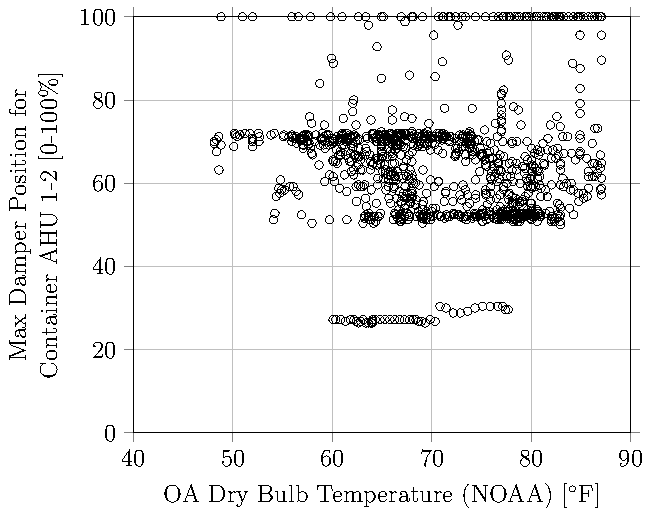
\includegraphics{Plots/MaximumDamperPosition-1-2.pdf} 
\caption{\MaxDampCaption{AHU-1-2}}
\label{fig:MaxDamperPositionforContainerAHU12vsOADryBulbTemperatureNOAA}
\end{figure}

\begin{figure}
\centering
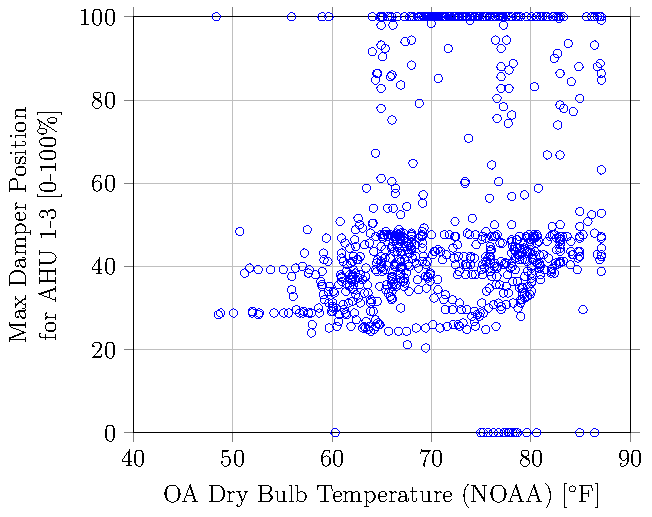
\includegraphics{Plots/MaximumDamperPosition-1-3.pdf}
\caption{\MaxDampCaption{AHU-1-3}}
\label{fig:MaxDamperPositionforContainerAHU13vsOADryBulbTemperatureNOAA}
\end{figure}


\begin{figure}
\centering
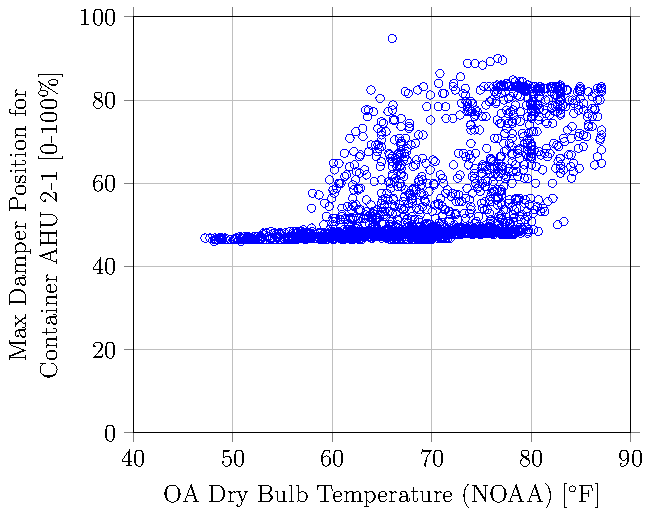
\includegraphics{Plots/MaximumDamperPosition-2-1.pdf}
\caption{\MaxDampCaption{AHU-2-1}}
\label{fig:MaxDamperPositionforContainerAHU21vsOADryBulbTemperatureNOAA}
\end{figure}

\begin{figure}
\centering
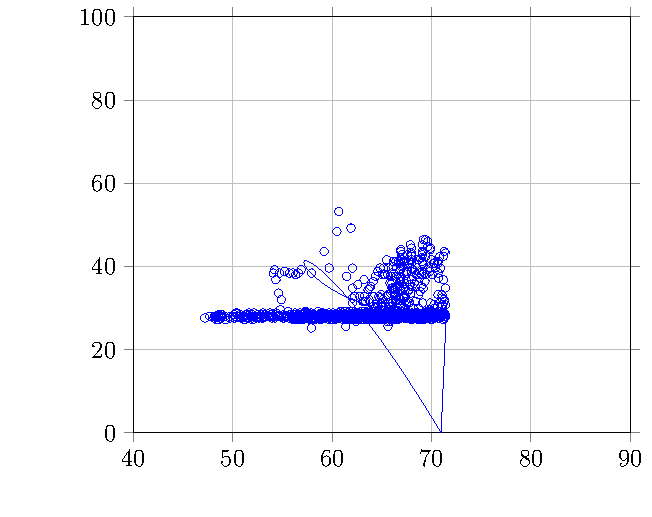
\includegraphics{Plots/2016-06-06-1427-MaxDamperPositionforContainerAHU22vsOADryBulbTemperatureNOAA.pdf}
\caption{\MaxDampCaption{AHU-2-2}}
\label{fig:MaxDamperPositionforContainerAHU22vsOADryBulbTemperatureNOAA}
\end{figure}

\begin{figure}
\centering
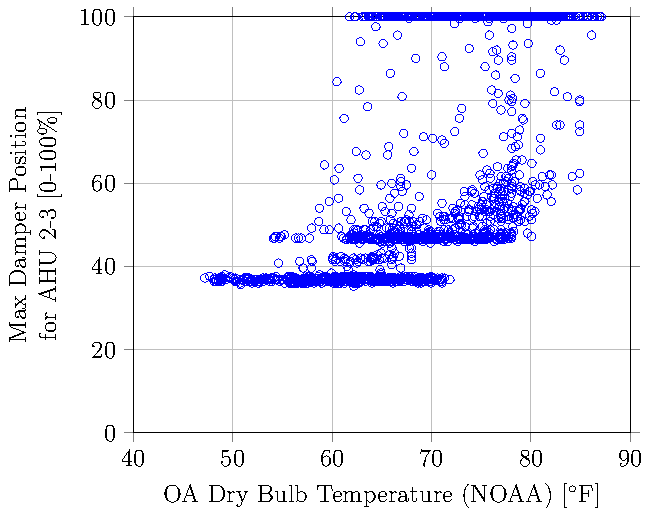
\includegraphics[]{Plots/2016-06-06-1454-MaxDamperPositionforContainerAHU23vsOADryBulbTemperatureNOAA.pdf}
\caption{\MaxDampCaption{AHU-2-3}}
\label{fig:MaxDamperPositionforContainerAHU23vsOADryBulbTemperatureNOAA}
\end{figure}


\subsection{Critical Zones for NCTM}

An investigation into the critical zones based on historical data was
completed. 15 minute interval data from Jan. 1, 2016 through Jun. 1,
2016 was used to check which damper positions were most open at a given
timestamp. \tableref{} \ref{tab:AHU12CriticalZone} shows the results of
this analysis. In all five of the applicable air handling units, there
is a damper that is critical at least 59\% of the time. 

%% Comes from file 2016-06-08-1603-CriticalZoneAnalysis.xlsx
%% Run from 2016-01-01 to 2016-06-01.
%% Assumes that the AHU is on. 
\begin{table}
\centering
\caption{Percentage of time that different terminal units for various AHUs were the most open during the period of Jan. 1, 2016 - Jun. 1, 2016.}
\label{tab:AHU12CriticalZone}
\begin{tabular}{@{}llll@{}}
\toprule
AHU                        & Unit       & Count of Max & Percent as Critical \\ \midrule
\multirow{3}{*}{AHU-1-2}   & FPVAV-1-8  & 3,518        & 68\%                \\
                           & FPVAV-1-9  & 1,281        & 25\%                \\
                           & 2 others   & 354          & 7\%                 \\ \midrule
\multirow{3}{*}{AHU-1-3}   & FPVAV-1-5  & 2,331        & 59\%                \\
                           & FPVAV-1-4  & 1,006        & 25\%                \\
                           & 4 others   & 622          & 15\%                \\ \midrule
\multirow{3}{*}{AHU-2-1}   & FPVAV-2-1  & 10,965       & 79\%                \\
                           & FPVAV-2-2  & 2,648        & 19\%                \\
                           & FPVAV-2-3  & 258          & 2\%                 \\ \midrule
\multirow{3}{*}{AHU-2-2}   & FPVAV-2-18 & 10,003       & 72\%                \\
                           & FPVAV-2-14 & 3,171        & 23\%                \\
                           & 6 others   & 648          & 5\%                 \\ \midrule
\multirow{3}{*}{AHU-2-3}   & FPVAV-2-6  & 9,883        & 72\%                \\
                           & FPVAV-2-11 & 3,743        & 27\%                \\
                           & FPVAV-2-10 & 184          & 1\%                 \\ \midrule
\end{tabular}
\end{table}


\subsection{Accuracy of Mechanical Specifications}

In the simplified analysis and modeling such as being proposed, it would be
ideal if the specifications in the mechanical drawings can be used
directly.  One important parameter is the design flow rate for the
terminal unit.  \tableref{} \ref{tab:TerminalUnitInformation} shows the
design flow rates for all the series fan powered terminal units in the
NCTM building.  The results show that the design specifications were
sufficiently accurate.  All data that were available at the time
(October 6, 2015 through June 7, 2016) were analyzed to capture a large
number of timestamps (over 22,000 timestamps).  There are several
reasons for potential differences between the maximum measured flow and
the design flow rates in the mechanical drawings.  It may be the case
that the terminal unit was oversized and the design flow rate was never
necessary. There may be bias in the flow rate measurements.  

The largest percent difference and absolute difference between the
measured maximum flow rate and design value was for FPVAV-1-9. The
difference was due to less than 15 outliers in the data (out of over
20,000 data points in total), and if they were to be removed, the
maximum is in line with the design value of 1,200 CFM for the vast
majority of the data, as seen in \figref{}
\ref{fig:FPVAV19AIRVOLUMEvsFPVAV19DMPRCOMD}. 

%%See file: Batch Plots -- Mitch Dissertation N -- 2016-06-09 0942.xlsx
\begin{table}
\centering
\footnotesize
\caption{Comparison of design flow specifications to actual data.}
\label{tab:TerminalUnitDesignSpecCheck}
\begin{tabular}{@{}llrl@{}}
\toprule
AHU &  Terminal Unit & \parbox{1.5cm}{\centering  Flow\\(CFM)}  & \parbox{2.7cm}{Maximum Meas. \\  Flow (CFM)}  \\ \midrule
%%\parbox{2cm}{AHU-1-1 \\ (5 hp)} & \multicolumn{3}{l}{No boxes - Serves Teaching Module alone, Constant Fan} \\ \midrule
AHU-1-2           & FPVAV-1-7  & 1,400 & 1,496 \\ \cmidrule(r){2-4}
(5 hp)            & FPVAV-1-8  & 700   & 840   \\ \cmidrule(r){2-4}
                  & FPVAV-1-9  & 1,200 & 1,688 \\ \cmidrule(r){2-4}
                  & FPVAV-1-10 & 1,600 & 1,712 \\ \midrule
AHU-1-3           & FPVAV-1-1  & 1,480 & 1,676 \\ \cmidrule(r){2-4}
(7.5 hp)          & FPVAV-1-2  & 1,160 & 1,240 \\ \cmidrule(r){2-4}
                  & FPVAV-1-3  & 1,300 & 1,364 \\ \cmidrule(r){2-4}
                  & FPVAV-1-4  & 1,400 & 1,760 \\ \cmidrule(r){2-4}
                  & FPVAV-1-5  & 1,040 & 612   \\ \cmidrule(r){2-4}
                  & FPVAV-1-6  & 1,120 & 1,288 \\ \midrule
%%\parbox{2cm}{AHU-1-4 \\ (7.5 hp)} & \multicolumn{3}{l}{No boxes - Serves open atrium outside lecture halls, constant fan}  \\\midrule
AHU-2-1          & FPVAV-2-1  & 2,000 & 2,016 \\ \cmidrule(r){2-4}
   (7.5 hp)      & FPVAV-2-2  & 2,200 & 2,060 \\ \cmidrule(r){2-4}
                 & FPVAV-2-3  & 1,800 & 1,824 \\ \midrule
AHU-2-2          & FPVAV-2-9  & 2,400 & 2,448 \\ \cmidrule(r){2-4}
(10 hp)          & FPVAV-2-12 & 500   & 452   \\ \cmidrule(r){2-4}
                 & FPVAV-2-13 & 1,000 & 1,032 \\ \cmidrule(r){2-4}
                 & FPVAV-2-14 & 850   & 892   \\ \cmidrule(r){2-4}
                 & FPVAV-2-15 & 1,400 & 1,332 \\ \cmidrule(r){2-4}
                 & FPVAV-2-16 & 500   & 484   \\ \cmidrule(r){2-4}
                 & FPVAV-2-17 & 1,280 & 1,304 \\ \cmidrule(r){2-4}
                 & FPVAV-2-18 & 600   & 604   \\ \midrule
AHU-2-3          & FPVAV-2-4  & 2,000 & 1,944 \\ \cmidrule(r){2-4}
        (7.5 hp) & FPVAV-2-5  & 600   & 504   \\ \cmidrule(r){2-4}
                 & FPVAV-2-6  & 400   & 228   \\ \cmidrule(r){2-4}
                 & FPVAV-2-7  & 200   & 252   \\ \cmidrule(r){2-4}
                 & FPVAV-2-8  & 1,200 & 1,184 \\ \cmidrule(r){2-4}
                 & FPVAV-2-10 & 540   & 588   \\ \cmidrule(r){2-4}
                 & FPVAV-2-11 & 560   & 656   \\ \bottomrule
\end{tabular}
\end{table}

%%See file: Batch Plots -- Mitch Dissertation N -- 2016-06-09 0942.xlsx
\begin{figure}
\centering
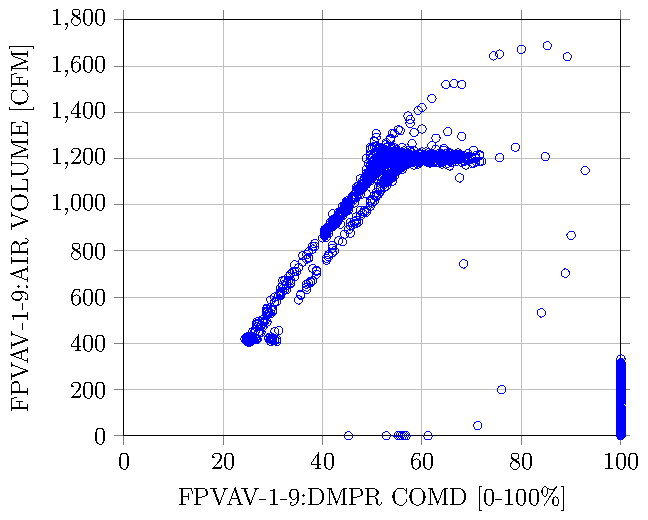
\includegraphics[]{Plots/2016-06-09-1038-FPVAV19AIRVOLUMEvsFPVAV19DMPRCOMD.pdf}
\caption{Damper position versus primary air flow for FPVAV-1-9.}
\label{fig:FPVAV19AIRVOLUMEvsFPVAV19DMPRCOMD}
\end{figure}


\section{Optimal Supply Air Temperature Results}\label{sec:OptimalSupplyAirTemperatureResults}

The methods described in the previous sections were used to determine
the optimal supply air temperature for various air handling units at the
NCTM building.  \figref{}
\ref{fig:2016-11-30-1004-AHU23MixedAirTemp-TikzData} shows the results
for AHU-2-3 during the work week from Monday, November 7, 2016 through
Friday, November 11, 2016.  During that week, the actual \(\sat\) hovered
between 58 and 60\(^\circ\)F. The optimal \(\sat\) was predicted using
different parameters for the simple fan curve exponent and plenum
temperature.  The optimization was completed using a fan exponent of 2
and 3, and the plenum temperature was assumed to be the room temperature
or assumed to be the static median values shown in \tableref{}
\ref{tab:plenumStatistics}.  Notice that even with the fan curve
exponent varying from 2 to 3, the optimal \(\sat\) is approximately
66\(^\circ\)F, 7\(^\circ\)F higher than the current operation. 

It is also apparent that for this case study that the optimal supply air
temperature is near the maximum of the search range.  The maximum
possible \(\sat\) searched is the minimum between the \(\mat\) and the
minimum calculated discharge temperature. The \(\sat\) cannot be above
the \(\mat\) because that would require heating in the air handling
unit, and cannot be above the minimum calculated discharge temperature
because then that particular zone would be starved for cooling capacity.
For the second floor air handling units, the minimum discharge
temperature is always less than the mixed air temperature indicating
that cooling will always be required.  

\figref{} \ref{fig:2016-11-30-0943-AHU21MixedAirTemp-TikzData} shows the
results for the same computations as \figref{}
\ref{fig:2016-11-30-1004-AHU23MixedAirTemp-TikzData}, but for AHU-2-1.
AHU-2-1 has 3 terminal units supporting a computer lab with higher
measured loads than the rest of the second floor.  The \(\mat\) is also
shown in \figref{} \ref{fig:2016-11-30-0943-AHU21MixedAirTemp-TikzData}
for reference. The optimal \(\sat\) appears to be higher than the
current operation, although not as much as the difference seen in
\figref{} \ref{fig:2016-11-30-1004-AHU23MixedAirTemp-TikzData}.


\figref{} \ref{fig:2016-11-16-1636-AHU22MixedAirTemp-TikzData} shows the
results for AHU-2-2.  In this case, the actual operation is near the
estimated optimal \(\sat\).

\begin{figure}
\centering
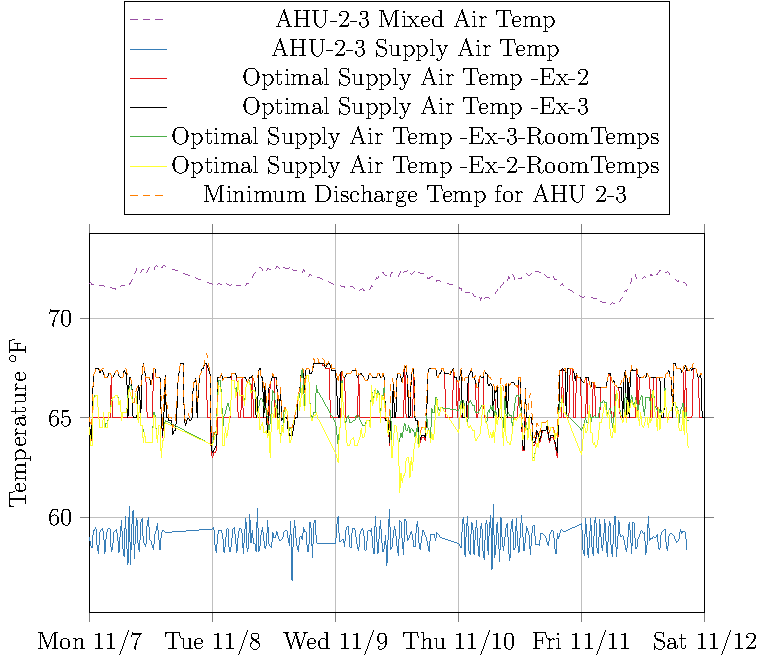
\includegraphics[]{Plots/2016-11-30-1004-AHU23MixedAirTemp-TikzData.pdf}
\caption{Optimal supply air temperature for AHU-2-3.}
\label{fig:2016-11-30-1004-AHU23MixedAirTemp-TikzData}
\end{figure}

\begin{figure}
\centering
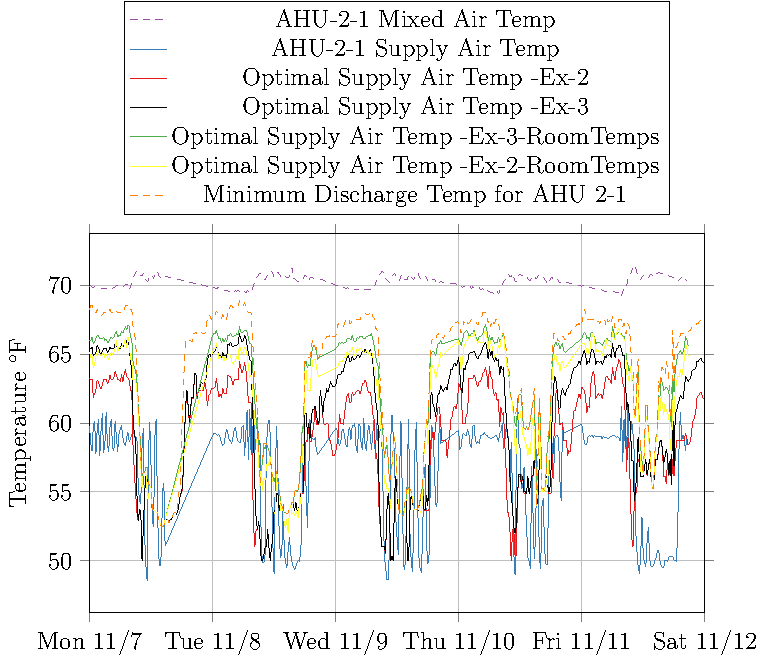
\includegraphics[]{Plots/2016-11-30-0943-AHU21MixedAirTemp-TikzData.pdf}
\caption{Optimal supply air temperature for AHU-2-1.}
\label{fig:2016-11-30-0943-AHU21MixedAirTemp-TikzData}
\end{figure}

\begin{figure}
\centering
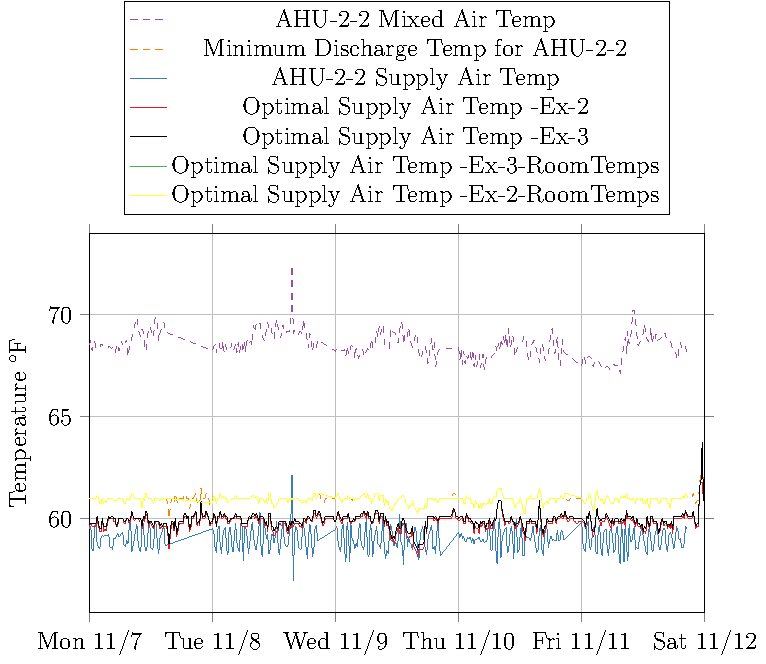
\includegraphics[]{Plots/2016-11-16-1636-AHU22MixedAirTemp-TikzData.pdf}
\caption{Optimal supply air temperature for AHU-2-2.}
\label{fig:2016-11-16-1636-AHU22MixedAirTemp-TikzData}
\end{figure}

\section{Savings Potential}

The potential for energy savings at the NCTM building was investigated
for the second floor AHUs. 

Energy savings were estimated for a period from June
1\textsuperscript{st} , 2016 to January 1\textsuperscript{st}, 2017.
Weekends, times when the AHUs were off, federal holidays, and times from
5:00 PM to 9:00 AM were all ignored. 

Also, since the estimation of the amount of reheat in terminal
units had a high uncertainty level, it was decided to ignore times in
which at least one of the reheat valves in the children terminal units
was open. In this sense, the only components to the AHU energy were the
cooling energy at the cooling coil and the fan energy. 

To provide a sense of the sensitivity to the assumed parameters in the
optimization, savings were determined using different exponents ranging
from 2 to 3 for the PLR curve, along with the plenum temperature assumed
to be the corresponding room temperature and the derived static
temperature shown in \tableref{} \ref{tab:plenumStatistics}. 

Based on the optimal supply air temperatures shown in Section
\ref{sec:OptimalSupplyAirTemperatureResults}, the potential savings in
AHU-2-1 and AHU-2-2 will be small since the systems are already
operating near optimally. However, the savings potential in AHU-2-3
appeared promising since there was approximately a \SI{5}{\degreeF}
difference between the operating supply air temperature and the
predicted optimal supply air temperature. 

\figref{}
\ref{fig:2017-01-24-1607-VariableTotalPowervsOADryBulbTemperatureNOAA}
shows the difference in the combined energy of the fan and cooling from
actual to optimal. Periods in which reheat was occurring was ignored
from the analysis. As expected, the energy use has a dependence on
\(\oat\). The optimal profile has a 3-Parameter cooling shape, as
described in \cite{ASHRAE2014}. 

The energy savings is primarily caused by increasing the supply air
temperature. There already was a reset programmed for AHU-2-3, but the
optimal reset would, in general, have a higher \(\sat\). 


\begin{figure}
\centering
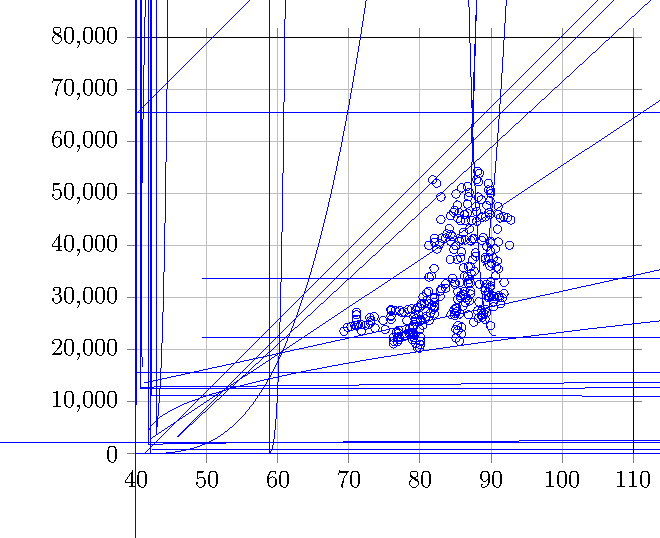
\includegraphics[]{Plots/2017-01-24-1607-VariableTotalPowervsOADryBulbTemperatureNOAA.pdf}
\caption{Energy savings for AHU-2-3 assuming a fan PLR exponent of 2 and plenum temperatures equal to the corresponding room temperature.}
\label{fig:2017-01-24-1607-VariableTotalPowervsOADryBulbTemperatureNOAA}
\end{figure}

\begin{figure}
\centering
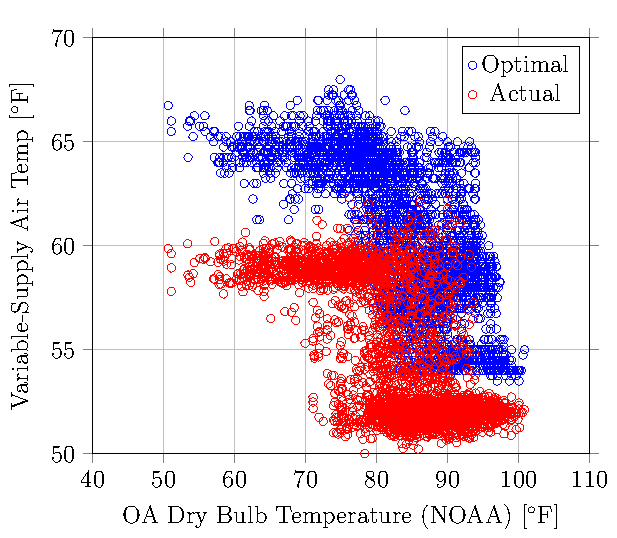
\includegraphics[]{Plots/2017-01-25-1121-VariableSupplyAirTempvsOADryBulbTemperatureNOAA.pdf}
\caption{Supply air temperature difference between actual and optimal.}
\label{fig:2017-01-25-1121-VariableSupplyAirTempvsOADryBulbTemperatureNOAA}
\end{figure}

% Table generated by Excel2LaTeX from sheet 'Sheet1'
\begin{table}[htbp]
  \centering
  \caption{Savings results, depending on model assumptions.}
  \begin{tabular}{C{2cm}C{4cm}R{2cm}R{2cm}r}
        \toprule
        Fan Exponent & Plenum Temperature Assumption & Actual (MMBTU) & Savings (MMBTU) & \% Savings \\
    \midrule
    2 & Room Temperatures  & 53.43 & 13.98 & 26\% \\
    3 & Room Temperatures  & 51.46 & 12.01 & 23\% \\
    2 & Static Temperature & 53.71 & 15.51 & 29\% \\
    3 & Static Temperature & 51.73 & 13.53 & 26\% \\
\bottomrule
    \end{tabular}%
  \label{tab:addlabel}%
\end{table}%


\section{Discussion}

Based on the previous results, several conclusions can be gathered that
relate to the proposed work.

The first is that it appears plausible that the ``zone load'' can be
reasonably estimated to provide useful optimization.  In fact, the
general relationship in the size of the thermal loads of the different
zones is more important than the precise value, of which the data
available is not capable of estimating. 

The second is that the design specifications from mechanical drawings
can be used as the first approximation for flows and power.  There was
general agreement between the terminal unit design flows and the actual
maximum realized flows at NCTM, as seen in \tableref{}
\ref{tab:TerminalUnitDesignSpecCheck}. 

A third conclusion is that the uncertainty in the optimal \(\sat\) is
small enough that in most cases, the current operation at NCTM does not
fall within the bounds.  In the cases shown in \figref{}
\ref{fig:2016-11-30-1004-AHU23MixedAirTemp-TikzData} through \figref{}
\ref{fig:2016-11-16-1636-AHU22MixedAirTemp-TikzData} the optimal
\(\sat\) was higher than the current operation. 
